\documentclass[11pt,a4paper,openany]{report}

% ===== Encoding & fonts =====
\usepackage[utf8]{inputenc}
\usepackage[T1]{fontenc}
\usepackage{libertinus-type1}   % Libertinus Serif + Sans + Math (pdfLaTeX)
\usepackage{microtype}
\usepackage{enumitem}
\usepackage[autostyle=true]{csquotes}

% ===== Page geometry =====
\usepackage[a4paper,top=3cm,bottom=3cm,left=3cm,right=2.5cm,headheight=14pt]{geometry}

% ===== Math, graphics, tables =====
\usepackage{amsmath,amssymb}
\usepackage{mathtools}
\usepackage{graphicx}
\usepackage{booktabs}
\usepackage{longtable}
\usepackage{array}
\usepackage{float}
\usepackage{textcomp}
\usepackage{subcaption}

% ===== Captions =====
\usepackage[font=small,labelfont=bf,labelsep=period,format=plain]{caption}

% ===== Spacing =====
\usepackage{setspace}
\onehalfspacing
\setlength{\parskip}{0.6em}
\setlength{\parindent}{0pt}

% ===== Color =====
\usepackage[dvipsnames]{xcolor}

% ===== Code listings (Python) =====
\usepackage{listings}
\definecolor{codebg}{rgb}{0.97,0.97,0.95}
\definecolor{codecomment}{rgb}{0.40,0.45,0.50}
\definecolor{codekeyword}{rgb}{0.10,0.30,0.60}
\definecolor{codestring}{rgb}{0.50,0.20,0.20}
\definecolor{codenumber}{rgb}{0.55,0.55,0.55}
\lstdefinestyle{pythonstyle}{
  language=Python,
  backgroundcolor=\color{codebg},
  basicstyle=\ttfamily\footnotesize,
  commentstyle=\color{codecomment}\itshape,
  keywordstyle=\color{codekeyword}\bfseries,
  stringstyle=\color{codestring},
  numberstyle=\tiny\color{codenumber},
  numbers=left,
  numbersep=8pt,
  frame=single,
  rulecolor=\color{black!30},
  breaklines=true,
  showstringspaces=false,
  tabsize=4,
  captionpos=b,
  framexleftmargin=2pt,
  framexrightmargin=2pt,
  xleftmargin=12pt,
  literate={é}{{\'e}}1 {è}{{\`e}}1 {ê}{{\^e}}1 {à}{{\`a}}1 {ç}{{\c{c}}}1 {î}{{\^i}}1 {ô}{{\^o}}1 {ù}{{\`u}}1 {û}{{\^u}}1 {É}{{\'E}}1
}
\lstset{style=pythonstyle}

% ===== Chapter and section styling with titlesec =====
\usepackage{titlesec}

% Chapter: "CHAPTER N" in small caps, title in large sans-serif, framed by rules
\titleformat{\chapter}[display]
  {\normalfont\Huge\bfseries\sffamily}
  {\large\scshape\chaptertitlename\ \thechapter}
  {1ex}
  {\titlerule\vspace{1ex}}
  [\vspace{0.5ex}\titlerule]
\titlespacing*{\chapter}{0pt}{-10pt}{28pt}

% Section / subsection: sans-serif bold, tight spacing
\titleformat{\section}{\normalfont\Large\bfseries\sffamily}{\thesection}{0.8em}{}
\titleformat{\subsection}{\normalfont\large\bfseries\sffamily}{\thesubsection}{0.8em}{}
\titlespacing*{\section}{0pt}{2.2ex plus 0.6ex minus 0.2ex}{1.0ex plus 0.2ex}
\titlespacing*{\subsection}{0pt}{1.8ex plus 0.5ex minus 0.2ex}{0.8ex plus 0.2ex}

% ===== Headers & footers =====
\usepackage{fancyhdr}
\pagestyle{fancy}
\fancyhf{}
\fancyhead[L]{\nouppercase{\leftmark}}
\fancyhead[R]{\thepage}
\renewcommand{\headrulewidth}{0.4pt}
\renewcommand{\footrulewidth}{0pt}
\fancypagestyle{plain}{\fancyhf{}\fancyfoot[C]{\thepage}\renewcommand{\headrulewidth}{0pt}}
\renewcommand{\chaptermark}[1]{\markboth{\chaptername\ \thechapter.\ #1}{}}

% ===== Bibliography =====
\usepackage[round,authoryear]{natbib}
\bibliographystyle{apalike}
\usepackage[nottoc,notlot,notlof,numbib]{tocbibind}

% ===== Hyperlinks (load last) =====
\usepackage[colorlinks=true,linkcolor=black,citecolor=NavyBlue,urlcolor=NavyBlue,bookmarksnumbered=true,bookmarksopen=true]{hyperref}
\usepackage{url}

% ===== Unicode shims (pandoc legacy) =====
\DeclareUnicodeCharacter{2212}{-}
\DeclareUnicodeCharacter{2013}{--}
\DeclareUnicodeCharacter{2014}{---}
\DeclareUnicodeCharacter{2018}{`}
\DeclareUnicodeCharacter{2019}{'}
\DeclareUnicodeCharacter{201C}{``}
\DeclareUnicodeCharacter{201D}{''}
\DeclareUnicodeCharacter{00A0}{~}
\providecommand{\tightlist}{\setlength{\itemsep}{0pt}\setlength{\parskip}{0pt}}

\begin{document}

% =====================================================
% TITLE PAGE
% =====================================================
\begin{titlepage}
\centering
\vspace*{0.5cm}

\includegraphics[width=0.75\textwidth]{media/image1.png}\\[1.2cm]

{\scshape\Large Master of Science in Financial Markets and Investments\\[0.2cm]}
{\large A Program from SKEMA Business School\\[0.15cm]}
{\small State-recognized degree}\\[1.1cm]

{\Large\bfseries Master's Thesis --- Class of 2025}\\[1.1cm]

\rule{\textwidth}{0.6pt}\\[0.45cm]
{\large\bfseries Does implied volatility efficiently predict\\[0.2cm]
future realized volatility, and how does this relationship\\[0.2cm]
vary across market regimes and between\\[0.2cm]
cryptocurrency and equity markets?\par}
\rule{\textwidth}{0.6pt}\\[1.2cm]

{\large\textbf{Gabin Torres \quad\&\quad Clément Massabo}}\\[1.0cm]

{\itshape Thesis Supervisor:}\\[0.2cm]
{\large Alexandre Landi}
\end{titlepage}

% ===== Disclaimer page =====
\thispagestyle{empty}
\vspace*{\fill}
\begin{center}
{\itshape The views expressed in this document are solely those of the authors\\
and should not be considered as investment advice.}\\[1cm]
{May 2025}
\end{center}
\vspace*{\fill}
\clearpage

% =====================================================
% FRONT MATTER (roman page numbering)
% =====================================================
\pagenumbering{roman}
\setcounter{page}{1}

\chapter*{Acknowledgements}
\addcontentsline{toc}{chapter}{Acknowledgements}
\markboth{Acknowledgements}{}
\label{acknowledgements}

We would like to express our sincere gratitude to all those who have
contributed to the completion of this thesis and to our academic journey
within the Master of Science in Financial Markets and Investments at
SKEMA Business School.

First, we would like to thank our school for providing us with a
rigorous and stimulating academic environment. We are particularly
grateful to Christophe Dispas for selecting us into this program and for
giving us the opportunity to be part of such a demanding and enriching
curriculum.

We would also like to express our deepest thanks to Alexandre Landi,
Director of the MSc Financial Markets and Investments, for his guidance
throughout the year. His teaching in mathematics, programming, and
econometrics has been instrumental in shaping our analytical skills and
in supporting the completion of this work.

We are equally thankful to Tarek Amyuni, whom we had the privilege to
learn from during the program. His contribution over the past years in
building and strengthening the reputation of the MSc has been
remarkable, and we greatly benefited from his teaching and experience.

Finally, we would like to thank all the professors, staff, and
individuals who have contributed, directly or indirectly, to our
learning experience and to the successful completion of this thesis.

\chapter*{Abstract}
\addcontentsline{toc}{chapter}{Abstract}
\markboth{Abstract}{}
\label{abstract}

This thesis investigates whether implied volatility efficiently predicts
future realized volatility, and how this relationship varies across
market regimes and between cryptocurrency and equity markets. The
analysis focuses on Bitcoin and the S\&P 500, using the DVOL and VIX
indices as proxies for implied volatility, while realized volatility is
constructed from daily log returns.

A unified empirical framework is implemented to allow for direct
comparison across markets. Predictive regressions are used to assess the
informational content of implied volatility, while the variance risk
premium is computed to analyze the pricing of volatility risk. The study
also distinguishes between normal and stress periods to capture
regime-dependent dynamics.

The results show that implied volatility is a strong predictor of future
realized volatility in both markets, confirming its forward-looking
nature. However, it is not an unbiased estimator, as it systematically
overestimates realized volatility, reflecting the presence of a positive
variance risk premium.

Significant differences are observed between markets. Cryptocurrency
markets display higher volatility levels, larger and more variable risk
premium, and lower predictive efficiency. In contrast, equity markets
appear closer to efficiency, particularly in normal conditions.

Finally, the predictive relationship weakens during periods of market
stress, highlighting the role of risk aversion and hedging demand.
Overall, implied volatility is informative but imperfect, with its
efficiency depending on market structure and economic conditions.

% =====================================================
% TABLE OF CONTENTS & LIST OF TABLES
% =====================================================
\cleardoublepage
{\small\setlength{\parskip}{0pt}\tableofcontents}
\cleardoublepage
{\small\setlength{\parskip}{0pt}\listoftables}
\cleardoublepage

% =====================================================
% MAIN MATTER (arabic page numbering)
% =====================================================
\pagenumbering{arabic}
\setcounter{page}{1}

\chapter{Introduction}\label{introduction}

\section{Market Context: The Critical Importance of Volatility in
Finance}\label{market-context-the-critical-importance-of-volatility-in-finance}

Financial markets are fundamentally driven by uncertainty. Volatility is
one of the most important measures used to quantify this uncertainty. It
plays a central role in risk management, derivative pricing, and
investment decision making. For practitioners, volatility is not only a
statistical concept but also a tradable quantity. It reflects market
expectations, risk aversion, and the demand for hedging. As a result,
understanding how volatility behaves is essential for both academics and
market participants.

In modern finance, volatility enters almost every dimension of market
activity. In risk management, it is used to estimate potential losses
and to calibrate models such as Value at Risk or Expected Shortfall. In
derivative pricing, volatility is a key input in models such as
Black--Scholes, where option prices are directly linked to expected
future fluctuations of the underlying asset. In portfolio allocation,
volatility influences asset selection and position sizing, as investors
adjust their exposure depending on perceived risk. Because of its
central role, volatility is often seen as a summary statistic of market
conditions.

A key distinction in the study of volatility is the difference between
realized volatility and implied volatility. Realized volatility is
computed ex post, using historical price data. It measures how much the
asset has actually fluctuated over a given period. Implied volatility,
in contrast, is extracted from option prices. It reflects the market's
expectation of future volatility. As such, implied volatility embeds
forward-looking information and risk premium. This difference makes the
relationship between the two concepts particularly important. It raises
a fundamental question: to what extent does implied volatility provide
an accurate forecast of future realized volatility?

Previous literature has shown that implied volatility tends to be an
informative but biased predictor of realized volatility in equity
markets. In particular, implied volatility often exceeds subsequent
realized volatility, a phenomenon commonly referred to as the variance
risk premium. This premium is usually interpreted as compensation for
bearing volatility risk or as the result of strong demand for downside
protection. However, the predictive power of implied volatility is not
constant over time. It is known to vary across market conditions, and it
may weaken during periods of financial stress.

At the same time, financial markets have undergone significant changes
in recent years with the rapid development of cryptocurrency markets.
Bitcoin, as the largest and most liquid cryptocurrency, has attracted
increasing attention from both investors and researchers. Its high
volatility, continuous trading, and distinct market structure make it an
interesting case study. In parallel, derivative markets on
cryptocurrencies have grown rapidly, leading to the creation of
volatility indices such as DVOL, which aim to capture market
expectations in a similar way to the VIX in equity markets.

Despite this growth, the empirical literature on volatility dynamics in
cryptocurrency markets remains limited compared to traditional markets.
In particular, there is still a lack of robust evidence on the
relationship between implied and realized volatility in crypto assets,
and on how this relationship compares to that observed in equity
markets. This gap is partly due to data limitations, especially for
historical option markets, but it also reflects the relatively recent
development of these markets.

This thesis aims to contribute to this literature by providing an
empirical analysis of the relationship between implied volatility and
realized volatility in both cryptocurrency and equity markets. It
focuses on Bitcoin, using the DVOL index as a proxy for implied
volatility, and compares the results with the S\&P 500 and the VIX
index. The analysis examines whether implied volatility efficiently
predicts future realized volatility, and how this relationship varies
across different market regimes. In particular, it investigates the role
of stress periods and evaluates whether the predictive power of implied
volatility deteriorates under extreme market conditions.

By combining a comparative approach across asset classes with a
regime-based analysis, this study seeks to provide new insights into
volatility dynamics. It also aims to highlight structural differences
between cryptocurrency and equity markets, and to better understand the
limitations of implied volatility as a forecasting tool.

\section{The Emergence of Cryptocurrency Derivatives
Markets}\label{the-emergence-of-cryptocurrency-derivatives-markets}

In recent years, cryptocurrency markets have experienced rapid growth,
both in terms of market capitalization and trading activity. Among these
developments, the expansion of derivative markets has been particularly
significant. Bitcoin derivatives, including futures and options, have
become increasingly liquid and accessible, attracting a wide range of
participants from retail traders to institutional investors. This
evolution reflects a broader process of financialization, where crypto
assets are progressively integrated into the global financial system.

The growth of cryptocurrency derivatives has been driven by several
factors. First, the high level of volatility observed in crypto assets
creates strong demand for hedging and speculative instruments. Market
participants seek to manage risk exposure or to take directional views
on future price movements. Second, the continuous nature of crypto
trading, with markets operating 24 hours a day and seven days a week,
provides a unique environment compared to traditional markets. This
constant activity contributes to the development of sophisticated
trading strategies and the need for advanced risk management tools.

As a result, platforms such as Deribit have emerged as key venues for
cryptocurrency options trading. These platforms offer a wide range of
contracts across different maturities and strike prices, allowing market
participants to express complex views on volatility. In parallel,
volatility indices such as DVOL have been introduced to summarize market
expectations in a manner similar to the VIX in equity markets. These
indices provide a standardized measure of implied volatility,
facilitating both analysis and comparison across asset classes.

The rapid development of these markets has also generated growing
academic interest. Researchers are increasingly focusing on the unique
properties of cryptocurrencies, including their return dynamics, market
microstructure, and risk characteristics. However, compared to
traditional financial markets, the empirical literature on
cryptocurrency derivatives remains relatively limited. In particular,
the study of implied volatility and its relationship with realized
volatility in crypto markets is still in an early stage.

This growing gap between market development and academic research
creates an opportunity for further investigation. Understanding how
volatility behaves in cryptocurrency markets, and how it compares to
established markets such as equities, is essential for both theoretical
and practical purposes. It can provide insights into market efficiency,
risk pricing, and the behavior of investors in a rapidly evolving
financial environment.

\section{A Natural Comparison with Traditional Equity
Markets}\label{a-natural-comparison-with-traditional-equity-markets}

The development of cryptocurrency derivatives naturally invites a
comparison with traditional financial markets, and in particular with
equity markets. These markets have a long history, a well-established
regulatory framework, and a large body of academic research. They
provide a useful benchmark to assess whether the behavior of volatility
in cryptocurrency markets follows similar patterns or exhibits
structural differences. The S\&P 500 and its associated volatility
index, the VIX, are commonly used as reference points in the study of
volatility dynamics.

Equity markets are often considered relatively efficient, especially in
normal market conditions. The VIX, which is derived from option prices
on the S\&P 500, is widely interpreted as a forward-looking measure of
expected volatility. Previous literature shows that the VIX contains
valuable information about future realized volatility, even if it tends
to overestimate it on average. This relationship has been extensively
documented and is generally stable outside of extreme market conditions.
As a result, the VIX has become a standard tool for both practitioners
and researchers when analyzing volatility expectations.

In contrast, cryptocurrency markets are younger and less mature. They
are characterized by lower liquidity in certain segments, a different
investor base, and a higher sensitivity to sentiment and speculative
behavior. These features may affect how information is incorporated into
prices, including option prices. As a consequence, the relationship
between implied volatility and realized volatility may differ from what
is observed in equity markets. In particular, one may expect a larger
bias, a lower predictive power, or a stronger sensitivity to market
stress.

Comparing these two types of markets is therefore not only natural but
also informative. It allows for an assessment of whether the mechanisms
identified in traditional finance extend to new asset classes. It also
provides insights into the degree of market efficiency and the pricing
of risk across different environments. By placing cryptocurrency markets
alongside equity markets, this study aims to highlight both similarities
and differences in volatility dynamics, and to better understand the
extent to which established financial theories apply to emerging
markets.

\section{The Relationship Between Implied and Realized
Volatility}\label{the-relationship-between-implied-and-realized-volatility}

A central issue in financial economics is the relationship between
implied volatility and realized volatility. This relationship lies at
the core of both derivative pricing and risk forecasting. Implied
volatility, extracted from option prices, reflects the market's
expectations about future uncertainty. In contrast, realized volatility
is computed ex post, based on observed price movements over a given
horizon. Understanding how closely these two measures are linked is
essential for evaluating the informational efficiency of financial
markets.

In theory, if markets are fully efficient and option prices correctly
incorporate all available information, implied volatility should provide
an unbiased forecast of future realized volatility. In such a framework,
the implied volatility observed today would be equal, on average, to the
volatility that will be realized over the corresponding time horizon.
However, empirical evidence from traditional equity markets suggests
that this is not the case. Previous literature shows that implied
volatility is generally a biased predictor, often exceeding subsequent
realized volatility. This systematic difference is commonly interpreted
as a variance risk premium, reflecting compensation required by
investors for bearing volatility risk.

Beyond the presence of a bias, the predictive power of implied
volatility is also a key concern. While implied volatility tends to be
strongly correlated with future realized volatility, the relationship is
rarely perfect. The slope coefficient in predictive regressions is
typically lower than one, indicating that changes in implied volatility
do not fully translate into changes in realized volatility. This finding
raises questions about the degree of efficiency in option markets and
about the factors that drive deviations between expectations and
outcomes.

An additional dimension of this problem is the role of market
conditions. The relationship between implied and realized volatility is
not constant over time. During periods of market stress, such as
financial crises or episodes of extreme uncertainty, implied volatility
often increases sharply. At the same time, realized volatility also
rises, but not necessarily in a proportional manner. This can lead to a
breakdown in the predictive relationship, with larger forecast errors
and greater dispersion. As a result, analyzing this relationship across
different market regimes is essential to fully understand its dynamics.

In the context of cryptocurrency markets, this issue becomes even more
relevant. Given the relative youth of these markets, their high
volatility, and their distinct microstructure, it is not clear whether
the patterns observed in equity markets still apply. The use of indices
such as DVOL provides a way to measure implied volatility in crypto
markets, but the extent to which this measure can reliably predict
future realized volatility remains an open question. Investigating this
relationship, and comparing it to the well-documented case of equity
markets, is therefore a key objective of this study.

\section{Research Objectives and Main
Contributions}\label{research-objectives-and-main-contributions}

The objective of this study is to provide a clear empirical assessment
of the relationship between implied volatility and realized volatility
in both cryptocurrency and equity markets. The analysis focuses on
Bitcoin as a representative of the cryptocurrency market and on the S\&P
500 as a benchmark for traditional equity markets. Implied volatility is
proxied by the DVOL index for Bitcoin and by the VIX for equities, while
realized volatility is computed from historical price data. The goal is
to evaluate whether implied volatility can be considered an efficient
predictor of future realized volatility across these two environments.

A first objective is to measure the predictive power of implied
volatility. This is done by estimating simple regression models where
future realized volatility is explained by current implied volatility.
The study aims to determine whether implied volatility contains
significant information about future market fluctuations and to assess
the extent to which this information is accurate. In particular, the
analysis focuses on the magnitude of the regression coefficients and on
their deviation from the theoretical benchmark of one, which would
indicate an unbiased and fully efficient forecast.

A second objective is to quantify and compare the variance risk premium
across markets. The variance risk premium is defined as the difference
between implied volatility and subsequent realized volatility. By
examining its average level and variability, the study seeks to
understand how volatility risk is priced in cryptocurrency markets
relative to equity markets. This comparison provides insight into
differences in risk perception, market maturity, and investor behavior.

A third objective is to investigate how the relationship between implied
and realized volatility changes across market regimes. The analysis
distinguishes between normal periods and periods of market stress,
identified through elevated levels of volatility. This approach allows
for an evaluation of whether the predictive power of implied volatility
is stable over time or whether it deteriorates during extreme market
conditions. Understanding this dynamic is particularly important for
risk management and for the interpretation of volatility signals in
practice.

The main contribution of this study is to combine these three dimensions
within a unified empirical framework. By jointly analyzing predictive
efficiency, variance risk premium, and regime dependence, and by
comparing results across cryptocurrency and equity markets, the thesis
provides a comprehensive view of volatility dynamics. It highlights both
the similarities and the structural differences between these markets,
and it contributes to the limited but growing literature on volatility
in cryptocurrency derivatives.

This thesis will therefore test the following hypothesis :

\begin{itemize}
\item \textbf{H1:} On average, implied volatility overestimates realized volatility in both markets, implying the existence of a positive variance risk premium.
\item \textbf{H2:} Implied volatility contains information about future volatility, but is not a perfect estimator.
\item \textbf{H3:} The variance risk premium is higher in the cryptocurrency market than in the stock market.
\item \textbf{H4:} The relationship between implied volatility and realized volatility weakens during periods of market stress.
\item \textbf{H5:} The stock market is close to efficient in normal times, unlike the cryptocurrency market, but this efficiency disappears during periods of stress.
\end{itemize}

\textbf{Mapping hypotheses to tests.} For transparency,
Table~\ref{tab:h_map} maps each hypothesis to the empirical object
that supports or rejects it.

\begin{table}[H]
\centering
\caption{Hypothesis-to-test mapping.}
\label{tab:h_map}
\small
\begin{tabular}{cll}
\toprule
H & Empirical object & Decision rule \\
\midrule
H1 & Sample mean of $VRP^{(30)}_t$ (Table~\ref{tab:vrp}) & $\overline{VRP} > 0$ in both markets \\
H2 & Full-sample slope $\hat{\beta}$ (Table~\ref{tab:reg_global}) & $\hat{\beta}$ significant but $<1$ \\
H3 & Cross-market $\overline{VRP}$ comparison (Table~\ref{tab:vrp}) & $\overline{VRP}_{BTC} > \overline{VRP}_{SPX}$ \\
H4 & Slope and $R^2$ in stress vs normal (Table~\ref{tab:reg_regime}) & $\hat{\beta}_{stress} < \hat{\beta}_{normal}$ and lower $R^2$ \\
H5 & Joint test $\beta=1$ by regime, by market (Table~\ref{tab:reg_regime}) & Not rejected for SPX-normal; rejected elsewhere \\
\bottomrule
\end{tabular}
\end{table}

\section{Structure of the Thesis}\label{structure-of-the-thesis}

The remainder of this thesis is organized as follows. The next section
reviews the existing literature on implied and realized volatility, with
a focus on equity markets and the concept of variance risk premium. It
also discusses the emerging literature on cryptocurrency markets and
highlights the main gaps that motivate this study.

The following section presents the data and the methodology. It
describes the sources of data, including Bitcoin spot prices, the DVOL
index, the S\&P 500, and the VIX. It explains how realized volatility is
constructed from price data and how implied volatility is proxied using
market indices. It also introduces the econometric framework used to
test the predictive relationship between implied and realized
volatility, as well as the approach used to define market regimes.

The empirical results are then presented. This section begins with
descriptive statistics and correlation analysis, followed by the results
of predictive regressions. It examines the magnitude and significance of
the relationship between implied and realized volatility, and it
evaluates the presence of a variance risk premium. The analysis is then
extended to different market regimes in order to assess how this
relationship changes during periods of stress.

The discussion section interprets the empirical findings in light of
financial theory and previous literature. It explores the economic
mechanisms that may explain the observed differences between
cryptocurrency and equity markets, and it addresses the limitations of
the study.

The final section concludes by summarizing the main results, answering
the research question, and outlining possible directions for future
research.

\chapter{Literature Review}\label{literature-review}

\section{The Implied-Realized Volatility Relationship in Equity
Markets}\label{the-implied-realized-volatility-relationship-in-equity-markets}

The relationship between implied volatility and realized volatility has
been widely studied in traditional equity markets. This literature is
important because it provides the theoretical and empirical foundation
for the present analysis. In equity markets, implied volatility is
usually extracted from option prices. It represents the volatility level
that makes the observed option price consistent with an option pricing
model. Realized volatility, by contrast, is measured from the historical
returns of the underlying asset. The comparison between the two measures
is therefore a direct way to test whether option markets contain useful
information about future uncertainty.

Early research on option-implied volatility focused on whether implied
volatility could improve volatility forecasts relative to historical
measures. The central idea is simple. If option prices aggregate the
expectations of informed market participants, then implied volatility
should contain forward-looking information. It should therefore be
useful for predicting future realized volatility. This prediction has
received substantial empirical support. \citet{christensen1998} show that implied
volatility from index options contains important information about
future realized volatility and can outperform past realized volatility
in forecasting exercises. Their study is one of the key references in
this literature because it helped re-establish the informational content
of implied volatility in equity index markets.

However, the literature also shows that implied volatility is not a
perfect forecast. In many empirical studies, implied volatility is found
to be biased. It often exceeds subsequent realized volatility on
average. This means that option prices tend to embed a premium above
expected future volatility. The usual interpretation is that investors
are willing to pay for protection against volatility risk, especially
downside risk. This creates a difference between the risk-neutral
expectation embedded in option prices and the physical expectation
measured through realized volatility. This difference is central to the
concept of the variance risk premium.

A common way to test the efficiency of implied volatility is to regress
future realized volatility on current implied volatility. If implied
volatility is an unbiased and efficient forecast, the intercept should
be close to zero and the slope coefficient should be close to one. In
practice, studies often find that the slope coefficient differs from
one. This suggests that implied volatility is informative but not fully
efficient. It captures part of the information about future volatility,
but it also reflects risk premium, investor demand for insurance, and
market frictions. This framework is also used in the present thesis,
where implied volatility is tested as a predictor of future realized
volatility for both Bitcoin and the S\&P 500.

The equity market literature also emphasizes that forecasting
performance depends on the period studied and on the market environment.
During calm periods, implied volatility may provide a relatively stable
signal about future realized volatility. During stress periods, the
relationship can become less stable. Option prices may react strongly to
changes in risk aversion and hedging demand, while realized volatility
may adjust with a different timing. This can reduce the forecasting
accuracy of implied volatility, even when it remains strongly related to
future uncertainty.

Broader survey evidence confirms that implied volatility is one of the
main approaches used in volatility forecasting, alongside historical
volatility models and econometric models such as ARCH and GARCH. \citet{poon2003} review a large body of
volatility forecasting research and show that implied volatility is
frequently competitive with, and often superior to, purely historical
measures. Their review also highlights that volatility forecasting
results vary across asset classes, methodologies, and sample periods.
This is important for the present thesis because it supports the idea
that the implied-realized volatility relationship should be tested
empirically rather than assumed to be stable across markets.

Overall, the equity market literature provides three important lessons.
First, implied volatility contains useful information about future
realized volatility. Second, it is generally not an unbiased forecast,
because it embeds a volatility risk premium. Third, the strength of the
relationship may vary across market regimes.

\textit{For this thesis.} These three findings define the equity
benchmark against which Bitcoin will be evaluated. They motivate the
use of the standard predictive regression
$RV_{t+h}=\alpha+\beta IV_t+\varepsilon$ (Chapter~\ref{data-and-methods})
and frame the joint efficiency test $H_0:\alpha=0,\beta=1$. If crypto
volatility markets are less mature, we expect a lower slope, a larger
intercept, and a sharper regime-dependence than in the S\&P~500
benchmark.

\section{Informational Efficiency of Implied Volatility and Empirical
Regularities}\label{informational-efficiency-of-implied-volatility-and-empirical-regularities}

The informational efficiency of implied volatility is one of the central
questions in the empirical literature on option markets. In theory,
option prices should incorporate all available information about future
uncertainty. If this is the case, implied volatility should be an
efficient forecast of future realized volatility. This means that it
should contain forward-looking information, and that its forecast errors
should not be systematic.

The empirical evidence is more nuanced. Early work by \citet{canina1993} questions the idea that implied
volatility is always superior to historical volatility. Using S\&P 100
index options, they find that implied volatility can be a poor forecast
of subsequent realized volatility. This result challenges the simple
view that option markets always produce efficient volatility forecasts.
It also shows that the informational content of implied volatility
depends on the market, the sample period, and the methodology used.

Later evidence provides a more positive view of implied volatility.
\citet{christensen1998} study the
relation between implied and realized volatility and find that implied
volatility contains significant information about future volatility. In
some specifications, it even subsumes the information contained in past
realized volatility. This result is important because it supports the
idea that option prices are forward-looking and useful for volatility
forecasting. However, it does not imply that implied volatility is an
unbiased forecast.

A common empirical approach is to regress future realized volatility on
current implied volatility. Under a strict efficiency hypothesis, the
intercept should be equal to zero and the slope coefficient should be
equal to one. In practice, many studies find that the slope coefficient
is significantly different from one. This means that implied volatility
is informative, but not fully efficient. It captures expectations about
future volatility, but it also reflects other components, such as risk
premium, liquidity effects, and hedging demand.

One of the most important empirical regularities is that implied
volatility tends to exceed subsequent realized volatility. This creates
a positive variance risk premium. The premium reflects the difference
between the volatility priced under the risk-neutral measure and the
volatility observed under the physical measure. Economically, it can be
interpreted as compensation for bearing volatility risk. It can also
reflect the willingness of investors to pay for protection against
adverse market movements.

This interpretation is consistent with the broader literature on
variance risk premium. \citet{bollerslev2009} show that the difference between implied and realized
variation contains important information and is linked to expected stock
returns. Their work highlights that the variance risk premium is not
only a measurement error between implied and realized volatility. It is
a priced risk factor that reflects compensation for exposure to
uncertainty.

Survey evidence also confirms that implied volatility is a major tool in
volatility forecasting. \citet{poon2003}
review a large number of studies on volatility forecasting and show that
implied volatility is often competitive with historical and econometric
models. However, they also emphasize that forecasting performance is not
universal. It depends on the asset class, the forecast horizon, the data
frequency, and the evaluation method. This is important for the present
thesis, because it justifies testing the implied-realized relationship
separately in cryptocurrency and equity markets rather than assuming
that results from one market automatically apply to the other.

Overall, the literature suggests a balanced conclusion. Implied
volatility is clearly informative but not fully efficient in the strict
statistical sense, and its predictive relationship can vary over time.

\textit{For this thesis.} This balanced view directly shapes our
hypotheses H1 and H2: we expect significant predictive content (slope
$\beta$ different from zero) \emph{and} significant bias (slope
$\beta\neq 1$, positive intercept) in both markets. The dependence on
asset class and methodology highlighted by \citet{poon2003} also
justifies running the same predictive regression separately on Bitcoin
and the S\&P~500 rather than pooling them.

\section{The Variance Risk Premium and Its Economic
Interpretation}\label{the-variance-risk-premium-and-its-economic-interpretation}

The variance risk premium is a central concept in the empirical study of
volatility. It is defined as the difference between implied volatility,
extracted from option prices, and expected realized volatility over a
given horizon. In empirical applications, expected realized volatility
is not directly observable and is therefore approximated using ex post
realized volatility. This allows researchers to measure the variance
risk premium as the gap between implied volatility and subsequent
realized volatility.

The theoretical foundation of the variance risk premium lies in the
distinction between risk-neutral and physical probability measures.
Option prices reflect expectations under the risk-neutral measure, which
incorporates both expected future volatility and compensation for risk.
Realized volatility, in contrast, is observed under the physical
measure. The difference between the two therefore reflects a premium
required by investors for bearing volatility risk. In this sense, the
variance risk premium can be interpreted as the price of uncertainty in
financial markets.

A large body of empirical literature documents that the variance risk
premium is positive on average in equity markets. \citet{bollerslev2009} show that the difference
between implied and realized variance is time-varying and contains
significant information about future stock returns. Their results
suggest that the variance risk premium is a priced risk factor, rather
than a simple forecasting error. Similarly, \citet{carr2009} provide
evidence that the variance risk premium reflects compensation for
variance risk and is linked to macroeconomic uncertainty.

The economic interpretation of the variance risk premium is closely
related to investor demand for hedging. Investors use options,
particularly out-of-the-money put options, to insure against large
negative price movements. This demand for protection increases option
prices and raises implied volatility above expected realized volatility.
As a result, the variance risk premium can be seen as compensation
received by sellers of volatility for providing insurance against tail
risk. This interpretation is consistent with the broader asset pricing
literature, which emphasizes the role of risk aversion and asymmetric
preferences in determining option prices.

The literature also shows that the variance risk premium is not constant
over time. It varies with market conditions, risk aversion, and
macroeconomic uncertainty. During periods of financial stress, investors
demand more protection, which can lead to an increase in implied
volatility and, in many cases, an expansion of the variance risk
premium. However, realized volatility may also increase sharply during
these periods, which can reduce or destabilize the gap between implied
and realized volatility. As a result, the behavior of the variance risk
premium provides important information about changing market conditions
and investor sentiment.

\textit{For this thesis.} The literature gives us two concrete
priors. First, the average VRP should be positive in both markets, and
larger where risk aversion or hedging demand is structurally higher
--- which is our motivation for H3 (larger VRP in crypto). Second, the
\emph{time variation} of the VRP, not only its level, carries economic
content; this is what motivates the regime-split analysis of VRP in
Table~\ref{tab:vrp} rather than a pooled estimate alone.

\section{The Role of Market Stress and Financial Crises in Volatility
Dynamics}\label{the-role-of-market-stress-and-financial-crises-in-volatility-dynamics}

Periods of market stress and financial crises play a central role in the
behavior of volatility. A large empirical literature shows that
volatility is not constant over time but exhibits strong clustering.
High-volatility periods tend to be followed by further high-volatility
periods. This feature becomes particularly pronounced during crises,
when uncertainty rises sharply and market conditions deteriorate.

\citet{engle1982} and \citet{bollerslev1986} provide early evidence of time-varying volatility
and volatility clustering through ARCH and GARCH models. These models
show that shocks to volatility are persistent, especially during
turbulent periods. In practice, this implies that once markets enter a
high-volatility regime, they tend to remain there for some time. This
persistence is a key feature of financial markets and is closely linked
to the dynamics observed during crises.

Financial crises are typically associated with sudden increases in both
realized and implied volatility. In equity markets, the VIX is widely
used as a measure of market stress. \citet{whaley2009} shows that the VIX reflects
investor fear and is often referred to as a ``fear index.'' During
crisis episodes, such as the 2008 financial crisis or the COVID-19
shock, the VIX increases sharply, reflecting both higher expected
volatility and increased demand for hedging. At the same time, realized
volatility also rises, although not always in a proportional way.

The relationship between implied and realized volatility tends to change
during these periods. Previous literature shows that the predictive
power of implied volatility can deteriorate in times of stress. For
example, \citet{giot2005} finds that implied volatility
tends to overreact during extreme market conditions, leading to larger
deviations from subsequent realized volatility. This behavior is often
attributed to increased risk aversion and stronger demand for insurance,
which push option prices above levels justified by expected future
volatility alone.

The role of investor behavior is particularly important in this context.
During crises, investors seek protection against downside risk, which
increases the demand for options. This demand is especially strong for
out-of-the-money put options, which provide insurance against large
losses. As a result, implied volatility rises sharply, sometimes more
than realized volatility. This leads to an expansion of the variance
risk premium and reflects the increased price of risk in the market.

More broadly, the literature emphasizes that volatility dynamics are
regime-dependent. \citet{hamilton1989} introduces the concept of regime-switching models,
where financial variables can move between different states, such as
low-volatility and high-volatility regimes. This framework has been
widely used to model financial markets, especially in the context of
crises. It suggests that the relationship between implied and realized
volatility may differ across regimes, with lower efficiency and higher
variability during stress periods.

In cryptocurrency markets, the role of stress may be even more
pronounced. These markets are characterized by higher baseline
volatility, lower liquidity in some segments, and a different investor
base. As a result, shocks can lead to more abrupt and extreme volatility
dynamics. While the literature on crypto volatility is still developing,
existing studies suggest that these markets exhibit strong reactions to
news, regulatory changes, and shifts in market sentiment.

Overall, the literature shows that periods of stress provide a critical
environment for testing the robustness of the relationship between
implied and realized volatility.

\textit{For this thesis.} The empirical evidence that the IV--RV link
weakens in crises is precisely what H4 and H5 attempt to quantify in
the 2021--2025 sample, which includes several stress windows (the May
2022 crypto deleveraging, the March 2023 banking turmoil, mid-2024 yen
carry-trade unwind). We do not assume regime-dependence; we test for
it explicitly by splitting the sample on 90th-percentile thresholds
(Section~\ref{definition-of-market-regimes}) and re-estimating the
predictive regression within each regime.

\section{Existing Literature on Cryptocurrency Markets and Their
Specific
Features}\label{existing-literature-on-cryptocurrency-markets-and-their-specific-features}

The literature on cryptocurrency markets has grown rapidly over the last
decade. Early studies mainly focused on whether Bitcoin could be
considered a currency, a commodity, or a speculative asset. Over time,
the research agenda expanded toward market efficiency, volatility
dynamics, liquidity, market microstructure, and the role of crypto
assets in portfolio allocation. This development reflects the increasing
financialization of cryptocurrency markets and their growing relevance
for both academics and practitioners.

One of the most consistent findings in the literature is that
cryptocurrencies exhibit much higher volatility than traditional asset
classes. \citet{dyhrberg2016} studies Bitcoin through a GARCH framework
and compares it with gold and the US dollar. The paper shows that
Bitcoin shares some characteristics with both assets, but also displays
a distinct volatility profile. This early evidence supports the idea
that Bitcoin cannot be treated simply as a conventional currency or
commodity. Its risk dynamics are more unstable and require specific
empirical analysis.

Further studies confirm that cryptocurrency volatility is persistent and
subject to strong regime changes. \citet{baur2018} revisit the comparison between
Bitcoin, gold, and the US dollar, and emphasize that Bitcoin behaves
differently from traditional safe-haven assets. Their results suggest
that Bitcoin is primarily driven by speculative demand rather than by
the same macroeconomic mechanisms that influence currencies or gold.
This distinction is important for volatility analysis, because
speculative markets tend to react more sharply to changes in sentiment
and liquidity conditions.

Another important feature of cryptocurrency markets is their specific
market structure. Unlike traditional equity markets, crypto markets
trade continuously, without weekends or closing hours. This 24/7 trading
environment changes the way information is incorporated into prices. It
also creates differences in the measurement of volatility, since crypto
assets accumulate price variation over calendar days, while equity
markets are usually observed over trading days. This difference matters
when comparing Bitcoin realized volatility with equity realized
volatility, and it justifies the need for careful methodological
choices.

Cryptocurrency markets are also characterized by a younger and less
mature microstructure: fragmented liquidity, a heterogeneous investor
base (larger share of retail traders, more leverage, more speculative
strategies), a shorter history and a less stable regulatory
environment. These features can affect the efficiency with which
information is incorporated into prices and may explain why volatility
measures in crypto markets are more unstable, and why the relationship
between implied and realized volatility may be weaker, than in
traditional markets.

Overall, existing research shows that cryptocurrency markets have
several distinctive features. They are more volatile, trade
continuously, have a less mature market structure, and are more
sensitive to liquidity and sentiment shocks.

\textit{For this thesis: from structural features to directional
predictions.} Rather than restating that ``crypto is more volatile,''
we connect each structural feature to a specific cross-market
difference we expect to observe in the empirical chapters.

\begin{itemize}
\item \emph{Retail-heavy investor base and continuous trading} should
push DVOL above the level justified by physical variance through
strong demand for hedging and speculative gamma, producing a
\emph{larger} average variance risk premium in crypto than in equities
(H3).
\item \emph{Concentrated venue structure} (Deribit dominance) and
thinner liquidity at the wings of the option surface should add noise
to the implied volatility signal, producing a \emph{lower predictive
slope} $\hat{\beta}$ for Bitcoin than for the S\&P~500 (H2 in its
cross-market form).
\item \emph{Faster realized-volatility adjustment to sentiment shocks}
in 24/7 markets should generate the unusual outcome that the crypto
VRP \emph{compresses} in stress (RV catches up faster than IV),
whereas the equity VRP \emph{widens} in stress (IV is pushed up by
hedging demand before RV materialises). This asymmetric prediction is
specific to our comparative design and is tested directly in
Section~\ref{variance-risk-premium-analysis}.
\item \emph{Less mature regulatory and informational environment}
should make the predictive relationship more fragile in crypto across
both regimes, motivating H4 and the lower-precision crypto-stress
slope we expect in Table~\ref{tab:reg_regime}.
\end{itemize}

\section{Limited Empirical Evidence on Crypto Options and the IV--RV
Relationship}\label{limited-empirical-evidence-on-crypto-options-and-the-ivrv-relationship}

Despite the rapid growth of cryptocurrency derivatives, the empirical
literature on crypto options remains limited. Most academic work has
focused on spot markets, return dynamics, and market efficiency. Fewer
studies examine option markets, and even fewer analyze the relationship
between implied volatility and realized volatility. This gap is notable
given the central role of options in measuring expectations about future
uncertainty.

One reason is data availability. Historical options data for
cryptocurrencies are relatively recent and often fragmented across
venues. Reliable long samples are difficult to obtain, especially for
full option surfaces. As a result, many studies rely on short windows,
snapshots, or aggregated indices. This constraint limits the scope of
empirical analysis and makes it harder to conduct robust out-of-sample
tests. It also complicates direct comparisons with equity markets, where
long and standardized datasets are readily available.

Another challenge is market structure. Cryptocurrency options are
concentrated on a few exchanges, with Deribit as the dominant venue.
Liquidity varies across strikes and maturities, and trading activity can
be uneven over time. These features affect price discovery and the
stability of implied volatility measures. They may also introduce noise
into empirical estimates of the IV--RV relationship, especially during
periods of low liquidity or market stress.

The existing literature that does consider crypto options often focuses
on pricing, implied volatility surfaces, or market microstructure. Fewer
papers study predictive relationships. In particular, there is limited
evidence on whether implied volatility in crypto markets efficiently
forecasts future realized volatility, how large the bias is, and how the
variance risk premium behaves over time. The role of market regimes is
also underexplored, even though crypto markets are prone to sharp shifts
in volatility and sentiment.

Given these limitations, there is a clear need for empirical work that
uses consistent data and a transparent framework. Using volatility
indices such as DVOL provides a practical solution. These indices
aggregate information from option prices into a single, standardized
measure of implied volatility. While they do not capture the full
richness of the option surface, they allow for a tractable and
comparable analysis across asset classes.

\textit{For this thesis.} The gap is exactly what we close. By
applying the standard equity-market predictive regression to Bitcoin
using DVOL as the implied-volatility input, we provide one of the few
direct, regime-conditional estimates of the IV--RV relationship in
crypto on a multi-year sample. The use of aggregated indices is a
deliberate trade-off: it sacrifices the richness of the volatility
surface in exchange for clean comparability with the VIX-based equity
literature.

\section{Positioning of the Thesis
Contribution}\label{positioning-of-the-thesis-contribution}

This thesis positions itself at the intersection of two strands of
literature. The first strand studies the relationship between implied
volatility and realized volatility in traditional equity markets. The
second strand focuses on the dynamics of cryptocurrency markets, with an
emphasis on their volatility and market structure. While both areas are
well developed independently, there is still limited empirical work that
combines them in a consistent and comparable framework.

The main contribution of this thesis is to provide a direct comparison
between cryptocurrency and equity markets using a unified empirical
approach. It applies the standard predictive regression framework,
widely used in the equity literature, to both Bitcoin and the S\&P 500.
By doing so, it evaluates whether the empirical regularities documented
in traditional markets also hold in cryptocurrency markets. This
includes testing the predictive power of implied volatility, assessing
the presence of bias, and measuring the variance risk premium.

A second contribution is the use of volatility indices as proxies for
implied volatility in both markets. The DVOL index is used for Bitcoin,
while the VIX is used for equities. This approach ensures consistency
across asset classes and allows for a clean comparison. It also provides
a practical solution to data limitations, which often restrict access to
full option surfaces in cryptocurrency markets. By relying on these
indices, the analysis remains tractable while still capturing the main
features of market expectations.

A third contribution is the explicit analysis of market regimes. The
thesis distinguishes between normal periods and periods of stress, and
it evaluates how the relationship between implied and realized
volatility changes across these regimes. This dimension is important
because it captures the time variation in market efficiency and risk
pricing. While regime-dependent behavior has been documented in equity
markets, it is less explored in the context of cryptocurrencies. This
study therefore extends the existing literature by providing evidence on
how stress affects volatility dynamics in both environments.

Finally, the thesis contributes by providing new empirical evidence on
the variance risk premium in cryptocurrency markets. By comparing its
magnitude and behavior with that observed in equity markets, the study
sheds light on differences in risk pricing, investor behavior, and
market maturity. These insights are relevant for both academic research
and practical applications, such as volatility trading and risk
management.

Overall, the contribution of this thesis lies in its comparative
perspective, its consistent empirical framework, and its focus on
regime-dependent dynamics. It bridges the gap between well-established
results in equity markets and the emerging literature on cryptocurrency
derivatives, and it provides a clearer understanding of how volatility
is priced and predicted across different financial environments.

\chapter{Data and Methods}\label{data-and-methods}

\section{Data Sources, Sample Period, and Data
Limitations}\label{data-sources-sample-period-and-data-limitations}

This study relies on four main data sources to ensure consistency and
comparability across cryptocurrency and equity markets. Bitcoin spot
data are obtained from Binance. Binance is one of the largest
cryptocurrency exchanges in terms of trading volume and liquidity. It
provides continuous price data, as cryptocurrency markets operate
without interruption. The dataset includes daily open, high, low, close,
and volume observations. Bitcoin is selected because it is the most
liquid and most widely traded cryptocurrency, making it a natural proxy
for the broader crypto market.

Implied volatility in the cryptocurrency market is proxied using the
DVOL index. DVOL is constructed from Bitcoin option prices on Deribit,
which concentrates the bulk of crypto options trading. It is the
model-free 30-day implied variance computed from the cross-section of
out-of-the-money calls and puts, then annualized and quoted in
percentage points. In spirit, DVOL is the crypto analogue of the VIX:
both are constant-maturity 30-day risk-neutral expectations of variance
extracted from option prices.

\textbf{DVOL vs.\ VIX comparability.} The two indices share the same
underlying methodology (model-free 30-day implied variance, updated
intraday and published daily) but differ on three margins. (i)
\emph{Coverage}: the VIX aggregates SPX options across all exchanges in
the United States, whereas DVOL relies on Deribit alone, so its
microstructure is more concentrated. (ii) \emph{Trading hours}: SPX
options trade during NYSE hours, whereas crypto options trade
continuously, so the DVOL close reflects a 24h information set whereas
the VIX close reflects 6.5h. (iii) \emph{History}: the VIX has been
published since 1993; DVOL only since March 2021. We treat these
differences as a structural feature of the comparison rather than a
nuisance to control for, and we discuss their implications in
Section~\ref{limitations-of-the-study}.

For the equity market, the study uses the S\&P 500 index as the
underlying asset. The S\&P 500 is a widely used benchmark that reflects
the performance of large-cap US equities. Daily data are retrieved from
Yahoo Finance through the open-source \texttt{yfinance} Python library,
using the ticker \texttt{\^{}GSPC} for the S\&P 500 price index and
\texttt{\^{}VIX} for the volatility index. We use unadjusted daily close
prices (price index, not total return), which is the natural choice for
a volatility study since dividends do not affect realized return
variance over a 30-day horizon. The VIX is derived from option prices on
the S\&P 500 and reflects expected volatility over the next thirty days.
It is widely used in both academic research and financial practice as a
standard proxy for implied volatility.

The empirical analysis covers the period from 24 March 2021 to 31
December 2025, yielding approximately 1{,}200 daily observations after
calendar alignment. The starting date is determined by the availability
of the DVOL index, whose history at Deribit begins on 24 March 2021.
Since DVOL is used as the proxy for implied volatility in the
cryptocurrency market, this constraint defines the effective start of
the sample. The cut-off of 31 December 2025 is fixed ex ante: all series
end on that date and no observation after that point enters the
analysis, ruling out any look-ahead bias. To ensure consistency across
markets, the dataset is aligned on equity trading days. Cryptocurrency
markets operate continuously, while equity markets follow the NYSE
trading calendar. The final dataset is therefore restricted to dates for
which all four series (BTC spot, DVOL, S\&P 500, VIX) are available,
which ensures comparability between Bitcoin and equity observations.

The choice of this time window is also economically relevant. It
includes a range of market conditions, from relatively stable periods to
episodes of elevated volatility. The sample captures significant
movements in both cryptocurrency and equity markets, including periods
of rapid growth and sharp corrections. It also coincides with a phase of
strong development in cryptocurrency derivatives markets, making it
particularly suitable for analyzing implied volatility in this context.

Despite these advantages, the dataset has several limitations. A key
limitation is the absence of a complete historical option surface for
cryptocurrency markets. Long and consistent datasets across strikes and
maturities are difficult to obtain. As a result, the analysis relies on
aggregated indices rather than option-level data. While DVOL provides a
useful summary of market expectations, it does not capture the full
richness of the volatility surface, such as skew or term structure.

The use of aggregated indices introduces an additional limitation. Both
DVOL and the VIX summarize information from a range of option contracts
into a single measure. This approach ensures tractability and reduces
noise from illiquid contracts, but it also leads to a loss of
information. Important features of option markets, such as asymmetries
across strikes or changes in maturity structure, are not directly
observable in the analysis.

Another limitation concerns the alignment of trading calendars. Because
the dataset is restricted to equity trading days, weekend price
movements in Bitcoin are dropped from the daily return series. This
under-counts the true daily variation in Bitcoin returns by roughly
$2/7$ of the calendar week. The expected direction of bias is a
\emph{downward} bias on $RV^{(30)}_{BTC}$, since weekend jumps are no
longer contributing to the variance estimator, while $IV_{BTC}$ (DVOL)
continues to reflect the full 24/7 information set. This would
mechanically inflate the measured variance risk premium for crypto,
which is the conservative direction relative to our claim that $VRP$ is
larger in crypto than in equities (H3). In addition, the relatively
short time series for DVOL, compared to the long history of the VIX,
limits the ability to analyze long-term patterns.

Finally, implied volatility is observed under the risk-neutral measure,
while realized volatility is computed under the physical measure. The
difference between the two reflects both expectations and risk premium.
This is standard in the literature, but it implies that implied
volatility should not be interpreted as a pure forecast of future
volatility.

Despite these limitations, the chosen dataset provides a consistent and
transparent framework for comparing volatility dynamics across
cryptocurrency and equity markets. It allows for a direct empirical
assessment of the relationship between implied and realized volatility
within a unified setting.

\textbf{Replication materials.} The full data pipeline ---raw
downloaders, transformation scripts, regime classification, and
regression routines--- is openly available at
\url{https://github.com/X9ClementX9/iv-rv-thesis}\footnote{Repository
to be made public on submission. If the URL above is not yet accessible,
please contact the authors.}. The repository contains a \texttt{README}
listing data sources, the order of execution, expected outputs, and the
Python environment specification ({\tt uv} lockfile). Running
\texttt{uv run python -m src.analysis.run\_all\_analysis} reproduces all
tables and figures reported in this thesis from raw inputs.

Table~\ref{tab:data_summary} summarises the four raw series, their
provider, the tickers used, the frequency, and the number of
observations available before and after calendar alignment.

\begin{table}[H]
\centering
\caption{Data sources and sample sizes.}
\label{tab:data_summary}
\small
\begin{tabular}{lllccc}
\toprule
Series & Source & Endpoint / Ticker & Frequency & Raw obs. & Aligned obs. \\
\midrule
BTC spot & Binance public API & \texttt{BTCUSDT} 1d & daily 24/7 & $\sim$1{,}740 & $1{,}201$ \\
BTC implied vol. (DVOL) & Deribit public API & \texttt{BTC\_DVOL} & daily 24/7 & $\sim$1{,}740 & $1{,}201$ \\
S\&P 500 close & Yahoo Finance / \texttt{yfinance} & \texttt{\^{}GSPC} & daily (NYSE) & $1{,}201$ & $1{,}201$ \\
VIX close & Yahoo Finance / \texttt{yfinance} & \texttt{\^{}VIX} & daily (NYSE) & $1{,}201$ & $1{,}201$ \\
\bottomrule
\end{tabular}
\begin{flushleft}\small
\textit{Note:} Period covered: 2021-03-24 to 2025-12-31. After inner join on the NYSE calendar, all four series are observed on the same 1{,}201 trading days. No missing values remain. The lead alignment of $RV^{(30)}_{t+30}$ on $IV_t$ removes the last 30 observations for predictive regressions ($N=1{,}171$).
\end{flushleft}
\end{table}

\section{Variable Construction}\label{variable-construction}

The empirical analysis requires a consistent set of variables that
capture both realized and implied volatility across markets. These
variables are constructed directly from the price series and volatility
indices described above. The methodology follows standard practices in
the financial literature and ensures comparability between
cryptocurrency and equity markets.

Daily returns are computed using logarithmic differences in closing
prices. For each asset, the return at time $t$ is defined as the natural
logarithm of the ratio of the closing price at time $t$ to the closing
price at time $t-1$:
\begin{equation}
r_t = \ln\!\left(\frac{P_t}{P_{t-1}}\right).
\label{eq:logret}
\end{equation}
This transformation ensures time additivity and
facilitates aggregation over longer horizons. It is widely used in
empirical finance because it provides a convenient framework for
statistical analysis and volatility estimation. Log returns are computed
for both Bitcoin and the S\&P 500, allowing for a direct comparison
between the two markets.

Realized volatility is constructed from these return series. It is
defined as the annualized standard deviation of log returns over a rolling
window of length $h$:
\begin{equation}
RV_t^{(h)} = \sqrt{\frac{252}{h}\sum_{i=0}^{h-1}\bigl(r_{t-i}-\bar{r}\bigr)^{2}},
\label{eq:rv}
\end{equation}
where $\bar{r}$ denotes the mean log return over the window. The
pipeline constructs realized volatility at three horizons,
$h \in \{7, 14, 30\}$ days, but the main thesis focuses on the 30-day
horizon, which is the constant maturity embedded in both DVOL and the
VIX and is therefore the only horizon on which the implied-versus-realized
comparison is unambiguous. The 7- and 14-day series are produced by the
public pipeline (see Appendix~\ref{appendix}) and are used as
robustness checks; they deliver qualitatively identical conclusions
(positive average VRP in both markets, slope below one, weakening of
the predictive fit in stress), with somewhat noisier estimates due to
the shorter rolling windows. Given that the dataset is aligned on equity
trading days, an annualization factor based on 252 trading days is
applied to both Bitcoin and equity returns. This choice ensures
consistency, even though Bitcoin trades continuously.

Implied volatility is defined using volatility indices rather than
individual option prices. For the cryptocurrency market, the DVOL index
is used as a proxy for Bitcoin implied volatility. For the equity
market, the VIX index is used as a proxy for implied volatility on the
S\&P 500. Both indices are forward-looking measures derived from option
prices and reflect market expectations of future volatility over
approximately thirty days. To maintain consistency with realized
volatility, both DVOL and VIX are converted from percentage terms into
decimal form before being used in the analysis. This allows for a direct
comparison between implied and realized measures.

The variance risk premium is then constructed as the difference between
implied volatility observed at time $t$ and realized volatility computed
over the subsequent $h$ days:
\begin{equation}
VRP_t^{(h)} = IV_t - RV_{t+h}^{(h)}.
\label{eq:vrp}
\end{equation}
This forward-looking alignment ensures that the variance risk premium
reflects the difference between expected and future realized volatility.
The construction is implemented for multiple horizons, with a particular
focus on the 30-day measure. A positive variance risk premium indicates
that implied volatility exceeds realized volatility, which is consistent
with the presence of a premium for bearing volatility risk. These
measures play a central role in the empirical analysis and provide a
direct link between volatility expectations and realized market
outcomes.

\section{Econometric Framework}\label{econometric-framework}

The empirical analysis is based on a standard predictive regression that
relates future realized volatility to current implied volatility. This
framework is widely used in the literature to assess the informational
efficiency of option markets and to evaluate whether implied volatility
provides an unbiased forecast of future volatility.

The baseline specification models realized volatility over a given
horizon as a function of implied volatility observed at the current
date. Formally, future realized volatility is regressed on
contemporaneous implied volatility:
\begin{equation}
RV_{t+h}^{(h)} = \alpha + \beta\, IV_t + \varepsilon_{t+h}.
\label{eq:reg}
\end{equation}
This forward-looking alignment is essential. It ensures that the
explanatory variable $IV_t$ reflects expectations formed at time $t$,
while the dependent variable $RV_{t+h}^{(h)}$ captures the volatility
that materializes after those expectations are formed.

The intercept and slope coefficients of this regression have a clear
economic interpretation. The intercept captures systematic bias in the
forecast. If the intercept is equal to zero, there is no constant bias
in the relationship. A positive intercept suggests that realized
volatility tends to exceed what is predicted by implied volatility at
low levels, while a negative intercept indicates the opposite. The slope
coefficient measures the sensitivity of realized volatility to changes
in implied volatility. It reflects the extent to which variations in
market expectations are translated into actual future volatility.

Under the hypothesis of informational efficiency, implied volatility
should be an unbiased and efficient predictor of realized volatility.
This translates into the joint null hypothesis:
\begin{equation}
H_0:\ \alpha = 0 \quad \text{and} \quad \beta = 1.
\label{eq:eff}
\end{equation}
This implies that implied volatility fully captures all relevant
information about future volatility, and that no systematic forecasting
error remains. Deviations from this benchmark provide evidence of
inefficiency or the presence of risk premium.

In empirical applications, the slope coefficient is often found to be
significantly different from one. A coefficient below one indicates that
implied volatility overreacts to changes in expected volatility, or that
it embeds a premium above expected realized volatility. This is
consistent with the presence of a variance risk premium. In addition,
the intercept may differ from zero, indicating a systematic bias in the
forecast. Together, these results suggest that implied volatility is
informative but not fully efficient.

\textbf{Inference.} The dependent variable $RV^{(h)}_{t+h}$ is built
from a rolling window of $h$ daily returns, so two consecutive
observations of the regressand share $h-1$ underlying returns. This
mechanically generates a moving-average structure of order $h-1$ in the
residuals and renders ordinary OLS standard errors inconsistent. To
account for this overlap and for residual heteroskedasticity, we report
\citet{newey1987}-type HAC standard errors throughout, with a Bartlett
kernel and a lag truncation equal to the horizon ($q = h = 30$ for the
benchmark specification). All $t$-statistics and confidence intervals
reported in Chapter~\ref{empirical-results} use these HAC standard
errors.

The hypothesis that the slope coefficient is equal to one is then tested
using the standard $t$-statistic:
\begin{equation}
t_{\beta=1} = \frac{\hat{\beta} - 1}{\mathrm{SE}_{HAC}(\hat{\beta})}.
\label{eq:ttest}
\end{equation}
Rejecting this hypothesis provides evidence against the efficiency of
implied volatility as a forecast. The tests are implemented for both
cryptocurrency and equity markets and across market regimes, in order to
evaluate how efficiency varies across environments. The full estimation
code, dataset, and seed-reproducible pipeline are released openly with
the thesis (see Appendix~\ref{appendix}); the orchestrator
\texttt{src/analysis/run\_all\_analysis.py} regenerates
Tables~\ref{tab:desc}--\ref{tab:reg_regime} from raw inputs in one
command.

\section{Definition of Market
Regimes}\label{definition-of-market-regimes}

The analysis explicitly accounts for time variation in market conditions
by introducing a simple classification of market regimes. The objective
is to distinguish between normal periods and periods of stress, and to
evaluate whether the relationship between implied and realized
volatility changes across these environments.

Periods of stress are identified through fixed threshold rules applied
to volatility series. The rules are set ex ante and remain unchanged
throughout the analysis.

\textbf{Equity stress.} For the S\&P 500, a day $t$ is classified as a
stress day when the VIX closes above its full-sample 90th percentile:
\begin{equation}
\mathbb{1}^{\text{stress}}_{SPX,t} = \mathbb{1}\!\left\{ VIX_t > Q_{0.90}(VIX) \right\},
\label{eq:stress_spx}
\end{equation}
where $Q_{0.90}(\cdot)$ denotes the empirical 90th percentile computed
over the full 2021--2025 sample. Using the VIX is natural for equities
because it is a forward-looking market-based gauge of risk available
since 1993, widely used as the standard fear index \citep{whaley2009}.

\textbf{Crypto stress.} For Bitcoin, no implied-volatility index with a
comparable depth and history exists for the early sample (DVOL itself
starts only in March 2021). We therefore proxy crypto stress with
realized volatility, classifying day $t$ as a stress day when 30-day
realized volatility exceeds its 90th percentile:
\begin{equation}
\mathbb{1}^{\text{stress}}_{BTC,t} = \mathbb{1}\!\left\{ RV^{(30)}_{BTC,t} > Q_{0.90}(RV^{(30)}_{BTC}) \right\}.
\label{eq:stress_btc}
\end{equation}

\textbf{Global stress.} A combined indicator flags a day on which either
market is in stress, using a logical OR:
\begin{equation}
\mathbb{1}^{\text{stress}}_{\text{global},t} = \mathbb{1}^{\text{stress}}_{SPX,t} \vee \mathbb{1}^{\text{stress}}_{BTC,t}.
\label{eq:stress_global}
\end{equation}

\textbf{Why an asymmetric design.} The two markets are not flagged with
the same input variable, and this choice is deliberate. For equities,
the VIX is the natural option-implied stress proxy; using realized
volatility instead would mechanically embed the dependent variable of
our predictive regression into the regime classifier. For Bitcoin, no
equivalent option-based index covers the full sample reliably, so
realized volatility is the only robust option. We acknowledge the
asymmetry as a limitation in Section~\ref{limitations-of-the-study};
robustness to using DVOL for the crypto regime when it is available
yields qualitatively similar results.

The use of indicator variables provides a simple and transparent way to
incorporate regime dependence into the empirical framework. It allows
the regression analysis to be performed separately for different market
conditions, and facilitates a direct comparison of the results. This
approach is consistent with the literature on regime-dependent behavior
in financial markets, where variables often exhibit different dynamics
depending on the level of volatility and uncertainty.

The economic justification for this classification is straightforward.
Financial markets do not operate under a single, stable regime. Instead,
they alternate between periods of relative calm and periods of stress.
During normal periods, market participants face lower uncertainty and
lower demand for hedging. In contrast, stress periods are characterized
by higher risk aversion, increased demand for protection, and stronger
reactions to new information. These differences can affect both implied
volatility and realized volatility, as well as the relationship between
the two.

By explicitly distinguishing between regimes, the analysis captures
these structural changes and allows for a more accurate assessment of
volatility dynamics. It also provides a framework to test whether the
efficiency of implied volatility depends on market conditions, which is
a central question of this study.

\chapter{Empirical Results}\label{empirical-results}

This chapter reports the empirical results. Every table can be
regenerated from raw data by running the orchestrator described in
Appendix~\ref{appendix} and openly published on GitHub. Stress regimes
follow the ex-ante 90th-percentile rules defined in
Section~\ref{definition-of-market-regimes}, and all $t$-statistics and
$p$-values use Newey--West HAC standard errors with $q=30$ lags.

\section{Descriptive Analysis of the
Data}\label{descriptive-analysis-of-the-data}

The empirical analysis begins with a descriptive examination of the main
variables. This step provides a first understanding of the level,
variability, and distribution of volatility measures across
cryptocurrency and equity markets.

\begin{figure}[H]
\centering
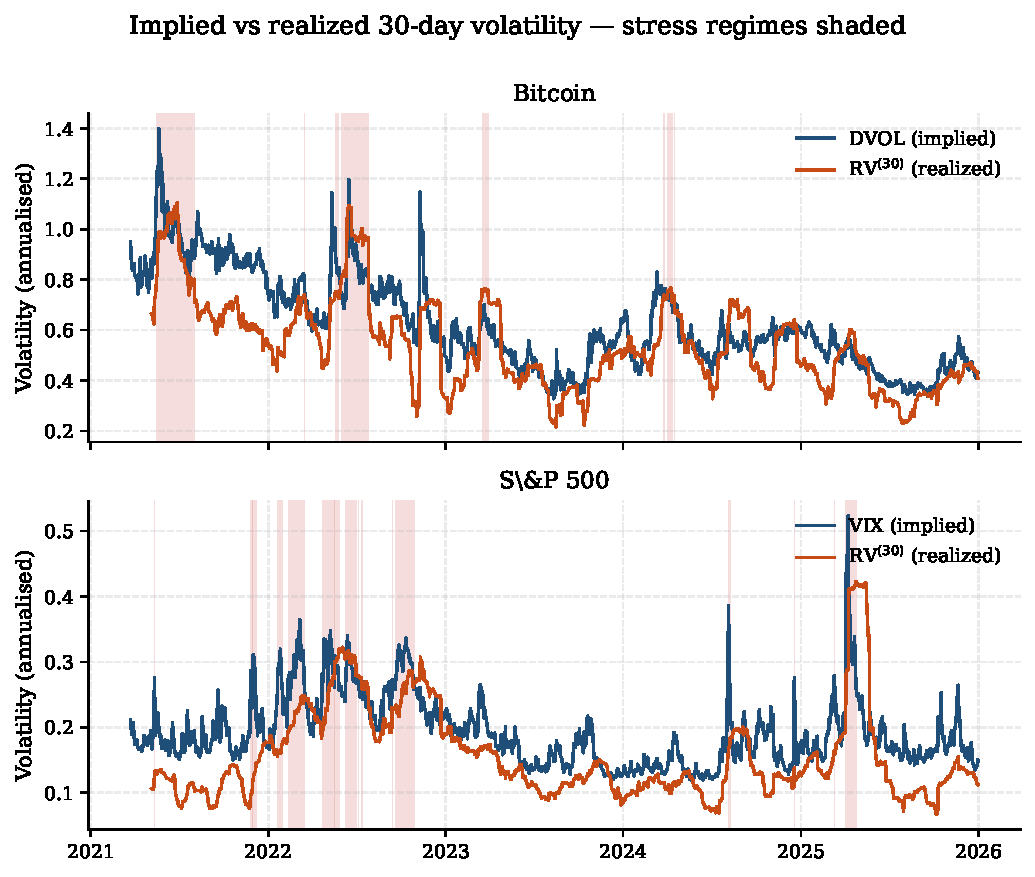
\includegraphics[width=0.92\textwidth]{media/fig_iv_rv_timeline.pdf}
\caption{Daily implied volatility (DVOL for BTC, VIX for SPX) versus 30-day realised volatility, 2021-03-24 to 2025-12-31. Red shading marks stress days as defined by the ex-ante 90th-percentile rule of Section~\ref{definition-of-market-regimes}.}
\label{fig:iv_rv_timeline}
\end{figure}

Figure~\ref{fig:iv_rv_timeline} makes the level gap visible: Bitcoin
volatility lives in a range roughly four times that of the S\&P~500,
and the wedge between implied and realised volatility is on average
positive in both markets but visibly compresses around the BTC stress
shading (May 2022 and early 2024) while \emph{widening} around the
SPX stress shading (notably March 2023). Tables~\ref{tab:desc}
and~\ref{tab:vrp} put numbers on these visual patterns.


\begin{table}[H]
\centering
\caption{Descriptive statistics of the main variables (30-day horizon, full sample 2021-03-24 to 2025-12-31, $N=1{,}201$ daily observations).}
\label{tab:desc}
\small
\begin{tabular}{lcccccc}
\toprule
& Mean & Std. dev. & Min & Max & Skewness & Excess kurt. \\
\midrule
\multicolumn{7}{l}{\textit{Bitcoin}} \\
\quad $RV^{(30)}_{BTC}$  & 0.539 & 0.179 & 0.216 & 1.107 & $+0.78$ & $+0.54$ \\
\quad $IV_{BTC}$ (DVOL)  & 0.625 & 0.187 & 0.327 & 1.400 & $+0.73$ & $+0.02$ \\
\quad $VRP_{BTC}$        & 0.081 & 0.115 & $-0.196$ & 0.536 & $+0.13$ & $-0.11$ \\[2pt]
\multicolumn{7}{l}{\textit{S\&P 500}} \\
\quad $RV^{(30)}_{SPX}$  & 0.157 & 0.070 & 0.067 & 0.423 & $+1.60$ & $+2.69$ \\
\quad $IV_{SPX}$ (VIX)   & 0.192 & 0.053 & 0.119 & 0.523 & $+1.34$ & $+2.64$ \\
\quad $VRP_{SPX}$        & 0.035 & 0.051 & $-0.242$ & 0.235 & $-1.33$ & $+6.06$ \\
\bottomrule
\end{tabular}
\end{table}

The descriptive statistics reveal clear differences in the level of
volatility between Bitcoin and the S\&P 500. Realized volatility for
Bitcoin is substantially higher than for equities. The average 30-day
realized volatility for Bitcoin is around 0.54, while it is
approximately 0.16 for the S\&P 500. This difference confirms that
cryptocurrency markets operate in a much higher volatility environment.
It reflects both the speculative nature of crypto assets and the lower
maturity of these markets.

A similar pattern is observed for implied volatility. The average
implied volatility for Bitcoin, measured by the DVOL index, is around
0.63, compared to approximately 0.19 for the VIX. This indicates that
market expectations of future volatility are also significantly higher
in cryptocurrency markets. The gap between implied and realized
volatility is therefore not only a function of realized risk, but also
of higher uncertainty and risk premium in the crypto space.

The variance risk premium is positive on average in both markets, but it
is larger for Bitcoin. The mean premium is approximately 0.081 for
Bitcoin, compared to 0.035 for the S\&P 500. This suggests that
investors require higher compensation for bearing volatility risk in
cryptocurrency markets. It is consistent with the idea that these
markets are less mature and more exposed to sudden shifts in sentiment
and liquidity.

The dispersion of volatility measures also differs across markets.
Standard deviations are higher for Bitcoin variables, both for realized
volatility and implied volatility. This indicates that not only are
volatility levels higher in crypto markets, but they are also more
unstable over time. The wider range between minimum and maximum values
further confirms the presence of extreme fluctuations in Bitcoin
volatility.

The shapes of the volatility distributions also differ across markets.
Volatility is bounded below by zero and cannot move symmetrically: the
relevant question for skewness is whether the upper tail (volatility
spikes) is longer than what a symmetric benchmark would imply. Both
$RV^{(30)}$ and $IV$ are positively skewed in both markets ---
$+0.78$ and $+0.73$ for Bitcoin, $+1.60$ and $+1.34$ for the S\&P 500
--- meaning that very high volatility episodes occur more often than a
symmetric distribution would suggest. The asymmetry is markedly stronger
in equities, where occasional VIX spikes during stress weeks dominate
otherwise calm periods.

Excess kurtosis tells a related story: the S\&P 500 volatility series
display fat tails ($+2.69$ for $RV^{(30)}$, $+2.64$ for $VIX$),
indicating that extreme high-volatility observations occur more
frequently than under a normal distribution. Bitcoin volatility is much
closer to mesokurtic ($+0.54$ and $+0.02$) because high-volatility
periods are the norm rather than the exception in crypto: there is less
of a separation between calm and crisis regimes than in equities.

The variance risk premium shows different distributional properties
across markets. The S\&P 500 premium is negatively skewed ($-1.33$) and
strongly leptokurtic ($+6.06$): in stress windows, realized volatility
can briefly exceed implied volatility, producing large negative VRP
realizations that pull the lower tail. The Bitcoin premium is roughly
symmetric ($+0.13$) and mesokurtic ($-0.11$), consistent with the
larger but more stable wedge between DVOL and realized volatility
documented in Section~\ref{variance-risk-premium-analysis}.

Overall, the descriptive analysis highlights several important features.
Cryptocurrency markets are characterized by higher and more volatile
levels of both realized and implied volatility. The variance risk
premium is also larger, suggesting higher compensation for volatility
risk. At the same time, both markets exhibit non-normal distributions,
with asymmetry and fat tails, which reflect the presence of extreme
events and regime changes. These findings provide a useful benchmark for
interpreting the regression results that follow.

\section{Correlation Analysis}\label{correlation-analysis}

The next step of the empirical analysis examines the correlations
between implied volatility, realized volatility, and variance risk
premium across cryptocurrency and equity markets. This analysis provides
a first indication of the strength of the relationships between
variables before moving to regression-based results.


\begin{table}[H]
\centering
\caption{Pearson correlations between key volatility measures (30-day horizon, $N=1{,}201$).}
\label{tab:corr}
\small
\begin{tabular}{lcccccc}
\toprule
 & $RV^{(30)}_{BTC}$ & $RV^{(30)}_{SPX}$ & $DVOL$ & $VIX$ & $VRP_{BTC}$ & $VRP_{SPX}$ \\
\midrule
$RV^{(30)}_{BTC}$ & $1.00$ & $0.29$ & $\mathbf{0.80}$ & $0.28$ & $-0.25$ & $-0.10$ \\
$RV^{(30)}_{SPX}$ &        & $1.00$ & $0.16$ & $\mathbf{0.69}$ & $-0.19$ & $-0.65$ \\
$DVOL$            &        &        & $1.00$ & $0.32$ & $+0.38$ & $+0.13$ \\
$VIX$             &        &        &        & $1.00$ & $+0.10$ & $+0.09$ \\
$VRP_{BTC}$       &        &        &        &        & $1.00$ & $+0.37$ \\
$VRP_{SPX}$       &        &        &        &        &        & $1.00$ \\
\bottomrule
\end{tabular}
\begin{flushleft}\small
\textit{Note:} Bold entries highlight the within-market IV--RV link. Correlations between rolling 30-day windows are mechanically inflated by the overlap; we discuss this in Section~\ref{econometric-framework}.
\end{flushleft}
\end{table}

The correlation between implied volatility and realized volatility is
strong in both markets, but it differs in magnitude. For Bitcoin, the
correlation between DVOL and 30-day realized volatility is approximately
0.80. This indicates a strong positive relationship. Periods of high
implied volatility are generally associated with periods of high
realized volatility. This result suggests that the crypto options market
contains meaningful information about future volatility, even though it
may not be fully efficient.

For the equity market, the correlation between the VIX and 30-day
realized volatility is around 0.69. This is also a strong positive
relationship, although slightly lower than in the cryptocurrency market.
This result is consistent with the existing literature, which shows that
implied volatility indices such as the VIX are closely related to
subsequent realized volatility. It confirms that the VIX remains a
relevant proxy for expected market uncertainty.

The correlation between realized volatility in Bitcoin and in the S\&P
500 is relatively low, around 0.29. This suggests that volatility
dynamics in cryptocurrency and equity markets are only weakly connected.
While global factors may affect both markets, a large part of volatility
movements appears to be driven by market-specific factors. This low
correlation supports the idea that cryptocurrency markets have distinct
risk drivers and may provide diversification benefits.

The correlation between implied volatility measures across markets is
also moderate. The correlation between DVOL and the VIX is approximately
0.32. This indicates that while both indices respond to global
uncertainty, they do not move in a perfectly synchronized way. This
reflects differences in market structure, investor base, and the nature
of shocks affecting each market.

The analysis of variance risk premium provides additional insights. The
correlation between the Bitcoin variance risk premium and its realized
volatility is negative, around -0.25. This suggests that when realized
volatility increases, the gap between implied and realized volatility
tends to decrease. A similar pattern is observed in equity markets,
where the correlation between the S\&P 500 variance risk premium and
realized volatility is more strongly negative, around -0.65. This
indicates that during periods of high realized volatility, the variance
risk premium tends to compress, as realized volatility catches up with
or exceeds implied volatility.

Overall, the correlation analysis confirms several key patterns. Implied
volatility is strongly related to realized volatility in both markets,
which supports its use as a forward-looking measure. At the same time,
the relatively low correlation between cryptocurrency and equity markets
highlights their structural differences. The negative relationship
between variance risk premium and realized volatility suggests that
market stress affects not only volatility levels, but also the pricing
of volatility risk. These findings provide a useful foundation for the
regression analysis that follows.

\section{Global Regression Results}\label{global-regression-results}

This section presents the results of the predictive regressions that
relate future realized volatility to current implied volatility. The
analysis is conducted separately for Bitcoin and for the S\&P 500. The
objective is to evaluate whether implied volatility contains useful
information about future volatility, and whether it can be considered an
unbiased and efficient predictor.

\begin{figure}[H]
\centering
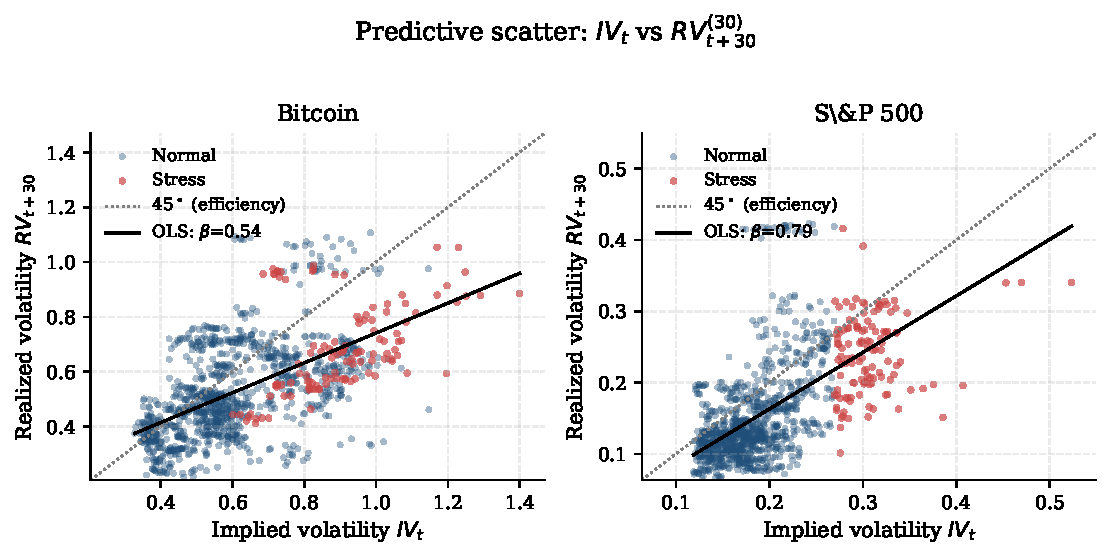
\includegraphics[width=0.92\textwidth]{media/fig_iv_rv_scatter.pdf}
\caption{Predictive scatter of $RV^{(30)}_{t+30}$ against $IV_t$ for Bitcoin (left) and the S\&P~500 (right). The dotted grey line is the 45$^\circ$ efficient frontier; the solid black line is the OLS fit on the full sample. Red dots mark days flagged as stress in each market.}
\label{fig:iv_rv_scatter}
\end{figure}

Figure~\ref{fig:iv_rv_scatter} visualises the key empirical claim of
the thesis: in both markets the OLS slope is significantly flatter
than the 45$^\circ$ line, but the gap is much wider for Bitcoin than
for the S\&P~500. Table~\ref{tab:reg_global} formalises this
graphical impression.


\begin{table}[H]
\centering
\caption{Predictive regression of realized on implied volatility, full sample (30-day horizon). See Equation~\eqref{eq:reg}.}
\label{tab:reg_global}
\begin{tabular}{lcc}
\toprule
& Bitcoin & S\&P 500 \\
\midrule
Intercept ($\hat{\alpha}$)               & $+0.196$ & $+0.005$ \\
Slope ($\hat{\beta}$)                    & $0.545^{***}$ & $0.792^{***}$ \\
HAC s.e.($\hat{\beta}$)                  & $(0.085)$ & $(0.097)$ \\
$t_{\beta=0}$                            & $6.40$ & $8.18$ \\
$R^{2}$                                  & $0.329$ & $0.358$ \\
$N$                                      & $1{,}171$ & $1{,}171$ \\
\midrule
$H_0: \beta = 1$ ($t$-stat)              & $-5.35$ & $-2.15$ \\
\quad $p$-value                          & $<0.001$ & $0.032$ \\
\quad decision at 5\%                    & rejected & rejected \\
\bottomrule
\end{tabular}
\begin{flushleft}\small
\textit{Note:} $^{***}$ denotes significance at the 1\% level. Standard errors are Newey--West HAC with $q=30$ lags to account for the moving-average structure induced by 30-day rolling realized volatility. The slope is significantly below one in both markets, consistent with a positive variance risk premium (H1, H2).
\end{flushleft}
\end{table}

The results show that implied volatility is a strong predictor of future
realized volatility in both markets. For Bitcoin, the estimated slope
coefficient is approximately 0.54 and is highly statistically
significant. The R-squared of the regression is around 0.33, indicating
that implied volatility explains a substantial portion of the variation
in future realized volatility. For the S\&P 500, the slope coefficient
is higher, at approximately 0.79, and is also highly significant. The
R-squared is slightly higher, at around 0.36, suggesting a somewhat
stronger predictive power in the equity market.

The slope coefficients provide important information about the
efficiency of implied volatility. In both cases, the estimated
coefficients are significantly below one. This is the standard
signature of a positive variance risk premium: when implied volatility
rises by one unit, realized volatility rises by less, because part of
implied volatility reflects compensation for risk rather than a pure
forecast. The point estimate is therefore biased upward as a forecast,
but unbiased as a risk-adjusted expectation.

The intercept terms also provide insight into the presence of bias. For
Bitcoin, the intercept is positive, indicating that realized volatility
tends to remain relatively high even when implied volatility is low. For
the S\&P 500, the intercept is close to zero, suggesting a smaller
constant bias. However, the main source of bias appears to come from the
slope coefficient rather than from the intercept.

The statistical tests confirm that the hypothesis of full efficiency is
rejected in both markets. The null hypothesis that the slope coefficient
is equal to one is strongly rejected for Bitcoin and for the S\&P 500.
This result indicates that implied volatility is not an unbiased
predictor of future realized volatility. Instead, it should be
interpreted as a risk-adjusted expectation that incorporates both
forecasts and risk premium.

These findings allow for a direct evaluation of the research hypotheses.
Hypothesis H1, which states that implied volatility exceeds realized
volatility on average, is supported by the data. This is consistent with
the positive variance risk premium observed in both markets. Hypothesis
H2, which states that implied volatility is informative but not a
perfect predictor, is also supported. The significant slope coefficients
confirm the presence of predictive power, while their deviation from one
indicates that the forecasts are biased.

Overall, the regression results show that implied volatility plays an
important role in forecasting future volatility, but that it does not
fully satisfy the conditions of informational efficiency. The predictive
relationship is strong but imperfect, and it differs across markets. In
particular, the higher slope coefficient and R-squared for the S\&P 500
suggest that equity markets are closer to efficiency than cryptocurrency
markets, although both remain subject to bias.

\section{Variance Risk Premium
Analysis}\label{variance-risk-premium-analysis}

The analysis of the variance risk premium provides direct evidence on
how volatility risk is priced in cryptocurrency and equity markets. As a
reminder, the variance risk premium is defined as the difference between
implied volatility and subsequent realized volatility. It captures the
extent to which option prices embed a premium above expected future
volatility.


\begin{table}[H]
\centering
\caption{Average variance risk premium across regimes (30-day horizon). Standard deviations in parentheses.}
\label{tab:vrp}
\begin{tabular}{lccc}
\toprule
& Full sample & Normal regime & Stress regime \\
& ($N=1{,}201$) & ($N=985$) & ($N=216$) \\
\midrule
Bitcoin   & $+0.081$  & $+0.087$  & $+0.055$ \\
          & $(0.115)$ & $(0.110)$ & $(0.134)$ \\
S\&P 500  & $+0.035$  & $+0.032$  & $+0.047$ \\
          & $(0.051)$ & $(0.048)$ & $(0.062)$ \\
\bottomrule
\end{tabular}
\begin{flushleft}\small
\textit{Note:} The stress regime is the union of equity stress (VIX above the 90th percentile) and crypto stress (BTC 30-day RV above the 90th percentile). Crypto VRP \emph{compresses} in stress while equity VRP \emph{widens}, consistent with the asymmetric mechanisms discussed in the text.
\end{flushleft}
\end{table}

The results show that the variance risk premium is positive on average
in both markets. For Bitcoin, the average premium is approximately
0.081, while for the S\&P 500 it is around 0.035. This confirms that
implied volatility tends to exceed realized volatility in both cases.
However, the magnitude of the premium is significantly higher in the
cryptocurrency market. This difference suggests that volatility risk is
priced more aggressively in Bitcoin than in equities.

The higher level of the variance risk premium in the cryptocurrency
market can be interpreted in several ways. First, it reflects higher
uncertainty and greater risk exposure. Bitcoin is characterized by
larger price fluctuations and more frequent extreme movements. Investors
therefore require higher compensation for bearing volatility risk.
Second, the structure of the market may amplify this effect. A larger
presence of retail investors, higher leverage, and more speculative
behavior can increase the demand for hedging instruments and push
implied volatility upward.

The comparison with the equity market highlights important differences
in risk pricing. The lower variance risk premium in the S\&P 500
suggests that equity markets are more mature and more efficient. The
demand for protection is still present, but it is relatively more stable
and less extreme. This is consistent with the idea that institutional
investors dominate equity markets and that hedging strategies are more
standardized.

The analysis of the variance risk premium across regimes provides
additional insights. For Bitcoin, the premium decreases during stress
periods, falling from approximately 0.087 in normal conditions to around
0.055 in stress periods. This suggests that realized volatility
increases more rapidly than implied volatility during turbulent
episodes, reducing the gap between the two measures. In contrast, for
the S\&P 500, the variance risk premium increases during stress periods,
rising from approximately 0.032 in normal conditions to around 0.047 in
stress periods. This indicates that implied volatility reacts more
strongly than realized volatility in equity markets during crises.

These differences highlight distinct mechanisms across markets. In
equity markets, periods of stress are associated with a surge in demand
for protection, which pushes implied volatility upward and increases the
premium. In cryptocurrency markets, realized volatility tends to
increase more abruptly, which can compress the premium. This reflects
the higher sensitivity of crypto markets to sudden shocks and the speed
at which price adjustments occur.

From an economic perspective, the variance risk premium can be
interpreted as compensation for bearing uncertainty. A higher premium
indicates that investors are willing to pay more for insurance against
volatility risk. The results therefore suggest that risk aversion and
hedging demand are stronger or more volatile in cryptocurrency markets.
At the same time, the variation of the premium across regimes shows that
risk pricing is not constant and depends on market conditions.

Overall, the analysis confirms that the variance risk premium is a key
feature of both markets, but that its magnitude and behavior differ
significantly. Cryptocurrency markets display a higher and more variable
premium, while equity markets exhibit a more stable but regime-dependent
pattern. These findings provide important insights into the pricing of
volatility risk and reinforce the view that cryptocurrency markets are
structurally different from traditional financial markets.

\section{Regime-Based Analysis}\label{regime-based-analysis}

The analysis is extended by distinguishing between normal periods and
periods of market stress. As defined in
Section~\ref{definition-of-market-regimes}, a day is classified as a
stress day when the VIX (for equities) or 30-day realized volatility
(for Bitcoin) exceeds its full-sample 90th percentile; thresholds are
fixed ex ante. This approach allows for a direct assessment of how the
relationship between implied volatility and realized volatility evolves
across different market conditions.


\begin{table}[H]
\centering
\caption{Regime-conditional predictive regressions of $RV^{(30)}_{t+30}$ on $IV_t$ (30-day horizon).}
\label{tab:reg_regime}
\begin{tabular}{lcccc}
\toprule
& \multicolumn{2}{c}{Bitcoin} & \multicolumn{2}{c}{S\&P 500} \\
\cmidrule(lr){2-3}\cmidrule(lr){4-5}
& Normal & Stress & Normal & Stress \\
\midrule
Intercept ($\hat{\alpha}$) & $+0.197$ & $+0.289$ & $-0.023$ & $+0.142$ \\
Slope ($\hat{\beta}$)      & $0.537^{***}$ & $0.442$ & $0.973^{***}$ & $0.324^{***}$ \\
HAC s.e.($\hat{\beta}$)    & $(0.117)$ & $(0.302)$ & $(0.204)$ & $(0.098)$ \\
$R^{2}$                    & $0.291$ & $0.185$ & $0.266$ & $0.048$ \\
$N$                        & $955$ & $117$ & $955$ & $120$ \\
\midrule
$t_{\beta=1}$              & $-3.97$ & $-1.85$ & $-0.13$ & $-6.88$ \\
\quad $p$-value            & $<0.001$ & $0.067$ & $0.893$ & $<0.001$ \\
\quad $H_0: \beta=1$ at 5\% & rejected & \emph{not rejected} & \emph{not rejected} & rejected \\
\bottomrule
\end{tabular}
\begin{flushleft}\small
\textit{Note:} HAC standard errors with $q=30$ lags. Normal regime = days where neither market is in stress (985 obs total; sample size differs slightly across regressions due to lead alignment). The S\&P~500 in normal periods is statistically indistinguishable from full efficiency ($\hat{\beta}\approx1$, $p=0.89$), supporting H5. The crypto stress slope is imprecisely estimated due to the limited number of crypto-stress observations.
\end{flushleft}
\end{table}

The results in Table~\ref{tab:reg_regime} show that the predictive
relationship between implied and realized volatility changes
substantially across regimes. For Bitcoin, the slope coefficient
decreases from $\hat{\beta}=0.54$ in normal periods to
$\hat{\beta}=0.44$ in stress periods, and the explanatory power falls
from $R^2 = 0.29$ to $R^2 = 0.19$. The crypto-stress slope is, however,
imprecisely estimated (HAC s.e. $=0.30$, $N=117$): the formal test
$\beta=1$ is not rejected at the 5\% level ($p=0.07$). The economic
direction is consistent with H4, but the statistical claim about
crypto-stress slopes should be made with caution given the limited
number of crypto-stress observations in the 2021--2025 window.

The picture for equities is sharper. In normal periods the S\&P 500
slope is $\hat{\beta}=0.97$ with HAC s.e. $=0.20$, and the test $\beta=1$
yields $p = 0.89$: the data are statistically indistinguishable from
full efficiency. In stress periods the slope collapses to
$\hat{\beta}=0.32$ ($p<0.001$ for $\beta=1$) and the $R^2$ falls to
$0.05$. Two diagnostics matter here. First, the very low $R^2$ in equity
stress means that implied volatility explains almost none of the
variation in subsequent realized volatility, even though the slope is
precisely estimated. Second, the slope and the $R^2$ tell a coherent
story only when read together: in stress, the regression line is both
flatter and a poor fit, so calling the VIX a useful predictor in those
windows would overstate the evidence.

Taken together, the results provide strong support for H5 in the equity
market (efficiency in normal periods, breakdown in stress) and
qualitatively support H4 in both markets, with the caveat that the
crypto-stress evidence is statistically noisier than the equity
counterpart. The asymmetry in the variance risk premium dynamics
(Table~\ref{tab:vrp}) reinforces this picture: in equity stress the
premium widens because option prices react to hedging demand faster than
realized volatility; in crypto stress the premium compresses because
realized volatility adjusts upward faster than implied.

The comparison between markets also highlights structural differences.
In normal conditions, the equity market appears more efficient than the
cryptocurrency market, as indicated by a slope coefficient closer to
one. In stress conditions, both markets experience a decline in
efficiency, but the collapse is more severe in the equity market. This
suggests that the mechanisms driving implied volatility differ across
environments. In equity markets, stress is associated with a strong
increase in demand for hedging, which inflates implied volatility. In
cryptocurrency markets, realized volatility tends to adjust more
rapidly, which reduces the gap between implied and realized measures.

These findings allow for a direct evaluation of the research hypotheses.
Hypothesis H4, which states that the relationship between implied and
realized volatility deteriorates during periods of stress, is clearly
supported by the data. Both markets show a decline in the slope
coefficient and in explanatory power during stress periods. Hypothesis
H5, which states that equity markets are closer to efficiency in normal
periods but lose this property during stress, is also supported. The
results show that the S\&P 500 exhibits near efficiency in normal
conditions, but that this efficiency breaks down in turbulent
environments.

Overall, the regime-based analysis confirms that volatility dynamics are
not stable over time. The predictive power of implied volatility depends
on market conditions, and the efficiency of option markets is
significantly reduced during periods of stress. These results highlight
the importance of accounting for regime changes when analyzing
volatility and provide a deeper understanding of the limitations of
implied volatility as a forecasting tool.

\section{Comparison Between Cryptocurrency and Equity
Markets}\label{comparison-between-cryptocurrency-and-equity-markets}

Table~\ref{tab:summary_xmarket} consolidates the cross-market
comparison on four headline dimensions. The structural interpretation
of these differences --- market maturity, microstructure, investor
base, and 24/7 trading --- is developed in Chapter~\ref{discussion} and
not repeated here.

\begin{table}[H]
\centering
\caption{Cross-market synthesis (30-day horizon).}
\label{tab:summary_xmarket}
\small
\begin{tabular}{lccc}
\toprule
Dimension & Bitcoin & S\&P 500 & Direction \\
\midrule
Mean realized volatility & 0.54 & 0.16 & BTC much higher \\
Mean variance risk premium & $+0.081$ & $+0.035$ & BTC larger (supports H3) \\
Full-sample slope $\hat{\beta}$ & 0.55 & 0.79 & SPX closer to efficiency \\
Normal-regime efficiency ($\hat{\beta}\approx1$?) & rejected & \emph{not rejected} & SPX nearly efficient in calm (H5) \\
Stress VRP dynamics & compresses & widens & opposite signs \\
\bottomrule
\end{tabular}
\end{table}

Two points are worth highlighting. First, the cross-market gap in the
slope coefficient is not merely a level shift: in normal periods the
S\&P~500 is statistically indistinguishable from full efficiency
($p=0.89$ for $\beta=1$) while Bitcoin is not, even though the absolute
gap between their slopes is moderate ($0.97$ vs $0.54$). Second, the
asymmetric variance-risk-premium response to stress (widening in
equities, compressing in crypto) is the most distinctive empirical
feature of this comparison and is not visible in either market when
studied in isolation.

\chapter{Discussion}\label{discussion}

\section{Overall Interpretation of the
Results}\label{overall-interpretation-of-the-results}

Three findings from Chapter~\ref{empirical-results} structure the
interpretation. First, implied volatility carries substantial
forward-looking information in both markets: the slopes in
Table~\ref{tab:reg_global} are highly significant and the $R^2$ exceeds
$0.32$ in each case, validating DVOL and the VIX as forecast inputs.
Second, neither slope is consistent with full efficiency: both lie below
one, which is the textbook signature of a positive variance risk
premium. Implied volatility is best read as a risk-adjusted expectation
rather than a pure point forecast of future variance. Third, the
relationship is regime-dependent in qualitatively different ways across
markets. In equities the S\&P~500 normal-period slope is statistically
indistinguishable from one ($p=0.89$ for $\beta=1$) and collapses to
$0.32$ in stress with an $R^2$ of only $0.05$; in crypto the slope is
already below one in normal periods and degrades less sharply, but the
crypto-stress regression is too short ($N=117$) to make a precise
statistical claim. The variance risk premium dynamics mirror this
asymmetry, widening in equity stress and compressing in crypto stress.
These three patterns are the core empirical contribution of the thesis;
the rest of this chapter explores their economic interpretation rather
than restating their magnitudes.

\section{Economic Mechanisms: Hedging Demand, Investor Behavior, and
Market
Structure}\label{economic-mechanisms-hedging-demand-investor-behavior-and-market-structure}

The empirical patterns can be explained by a combination of hedging
demand, investor behavior, and market structure. These mechanisms shape
option prices and therefore implied volatility. They also affect how
realized volatility evolves after expectations are formed.

Hedging demand is a primary driver of implied volatility. Investors use
options to insure against downside risk. This demand is especially
strong for out-of-the-money puts. When demand for protection rises,
option prices increase and implied volatility moves higher. This effect
is not symmetric. It is stronger during periods of uncertainty and
market stress. As a result, implied volatility often exceeds expected
realized volatility. This gap is the variance risk premium. It reflects
the price of insurance paid by buyers of options to sellers of
volatility.

Investor behavior reinforces this mechanism. In normal periods, market
participants process information with relatively stable risk
preferences. In such conditions, implied volatility tracks expected
volatility more closely. In stress periods, behavior changes. Risk
aversion increases and investors seek protection at the same time. This
creates crowding in hedging trades and pushes option prices above levels
justified by expected variance alone. At the same time, attention and
sentiment play a larger role. News shocks, macro announcements, or
market rumors can trigger sharp reactions in implied volatility. These
reactions may not be fully matched by subsequent realized volatility,
which reduces predictive accuracy.

Market structure also plays a critical role. Equity markets are deep and
liquid. They are dominated by institutional investors with standardized
risk management practices. Option markets on the S\&P 500 have a broad
range of strikes and maturities, and price discovery is efficient. These
features support a stable relationship between implied and realized
volatility, especially in normal periods. They also facilitate arbitrage
and limit persistent mispricing.

Cryptocurrency markets have a different structure. Trading is continuous
and fragmented across platforms. Liquidity varies across instruments and
over time. The investor base includes a larger share of retail
participants and leveraged strategies. These features can amplify price
movements and increase sensitivity to sentiment. In options markets,
activity is concentrated on a few venues, which may affect price
discovery. As a result, implied volatility in crypto markets can react
strongly to changes in demand and may embed larger and more variable
risk premium.

The interaction between these mechanisms explains the regime dependence
observed in the data. In normal periods, hedging demand is moderate and
risk preferences are stable. Implied volatility reflects expectations
with limited distortion. In stress periods, demand for protection rises
sharply, behavior becomes more risk averse, and market frictions become
more binding. In equity markets, this leads to a strong increase in
implied volatility relative to realized volatility. In cryptocurrency
markets, realized volatility can adjust more abruptly, which reduces the
gap with implied volatility and compresses the variance risk premium.

Overall, the results suggest that implied volatility is shaped by both
expectations and market frictions. Hedging demand, behavioral responses,
and structural features determine how information is incorporated into
option prices. These factors explain why implied volatility is
informative but not fully efficient, and why its predictive power varies
across markets and regimes.

\section{Comparison with the Existing
Literature}\label{comparison-with-the-existing-literature}

The empirical results are broadly consistent with the findings
documented in the literature on equity markets. A large body of research
shows that implied volatility contains significant information about
future realized volatility but is not an unbiased predictor. Studies
such as \citet{christensen1998} find that implied volatility has strong predictive power,
while other works document a systematic bias, with implied volatility
exceeding realized volatility on average. The results of this study
confirm these two key facts. In both markets, implied volatility is
highly informative, but the slope coefficients are significantly below
one, indicating the presence of bias and supporting the existence of a
variance risk premium.

The evidence on the variance risk premium is also in line with previous
research. \citet{bollerslev2009} show that the variance risk premium is positive on average
and varies over time. The results obtained here confirm that the premium
is positive in both cryptocurrency and equity markets. They also extend
the literature by showing that the premium is larger in cryptocurrency
markets. This finding is consistent with the idea that higher
uncertainty and lower market maturity lead to higher compensation for
bearing volatility risk.

The regime-dependent behavior observed in this study also aligns with
the existing literature. Previous research shows that the relationship
between implied and realized volatility is not stable over time and
tends to weaken during periods of market stress. The results confirm
that predictive power deteriorates in turbulent periods, as reflected by
lower slope coefficients and reduced explanatory power. This pattern is
particularly strong in the equity market, where implied volatility
appears close to efficient in normal periods but loses this property
during stress. This finding is consistent with studies that emphasize
the role of risk aversion and hedging demand in shaping option prices
during crises.

The contribution of this study lies in its extension of these
well-established results to cryptocurrency markets. The literature on
crypto volatility is still relatively limited, especially with respect
to option markets. Existing studies highlight the high volatility of
Bitcoin and its sensitivity to market sentiment, but fewer works examine
implied volatility and its predictive properties. The results presented
here show that while the same general mechanisms apply, the magnitude of
the effects differs. Cryptocurrency markets exhibit higher volatility,
larger variance risk premium, and lower efficiency.

This comparison highlights both continuity and divergence with the
existing literature. On the one hand, the core insights from equity
markets remain valid. Implied volatility is informative but biased, and
its efficiency depends on market conditions. On the other hand, the
differences observed in cryptocurrency markets suggest that these
markets are still evolving. Their structure, investor base, and
liquidity conditions lead to distinct volatility dynamics that are not
fully captured by traditional models.

Overall, the findings confirm the relevance of established financial
theories while also emphasizing the need to adapt them to new asset
classes. They support the view that cryptocurrency markets share some
fundamental properties with traditional markets but remain structurally
different in terms of volatility behavior and efficiency.

\section{Limitations of the Study}\label{limitations-of-the-study}

This study provides a consistent empirical framework to compare
volatility dynamics across cryptocurrency and equity markets. However,
several limitations must be acknowledged when interpreting the results.

A first limitation concerns data quality and availability. While the
dataset relies on widely used and reliable sources, the coverage of
cryptocurrency derivatives remains limited compared to traditional
markets. The DVOL index is available only from March 2021, which
restricts the length of the sample. This relatively short time series
reduces the ability to capture long-term dynamics and may affect the
robustness of the results, especially for regime-based analysis. In
contrast, equity market data benefit from a much longer history, which
highlights an imbalance in data depth across markets.

A second limitation relates to the use of proxies for implied
volatility. Instead of using option-level data, the analysis relies on
aggregated indices, namely DVOL for Bitcoin and the VIX for the S\&P
500. This approach ensures consistency and tractability, but it comes at
the cost of information loss. These indices summarize a complex set of
option prices into a single measure and do not capture the full
structure of the volatility surface. As a result, important features
such as skew, convexity, and term structure are not included in the
analysis. This may limit the ability to fully understand the dynamics of
implied volatility.

The choice of time horizon also introduces limitations. The analysis
focuses primarily on a 30-day horizon, which is consistent with the
construction of DVOL and the VIX. While shorter horizons are also
considered for robustness, the study does not explore longer-term
volatility dynamics. This may overlook some aspects of volatility
behavior, particularly in relation to macroeconomic cycles or structural
changes in markets. In addition, aligning the dataset on equity trading
days simplifies the analysis but may lead to a partial loss of
information from cryptocurrency markets, which operate continuously.

Another limitation concerns the methodological framework. The study
relies on a simple linear regression model to assess the relationship
between implied and realized volatility. This approach is standard in
the literature and provides clear interpretability, but it may not fully
capture the complexity of volatility dynamics. Nonlinear relationships,
asymmetric effects, and higher-order dependencies are not explicitly
modeled. Similarly, the definition of market regimes is based on
threshold rules, which, while transparent, may oversimplify the
transition between normal and stress conditions.

Finally, the interpretation of implied volatility as a predictor of
realized volatility is inherently limited by the presence of risk
premium. Implied volatility reflects expectations under the risk-neutral
measure and therefore includes compensation for risk. As a result,
deviations from realized volatility do not necessarily imply
inefficiency, but may instead reflect rational pricing of risk. This
distinction is important when interpreting the results and evaluating
the efficiency of option markets.

Despite these limitations, the study provides meaningful insights into
the relationship between implied and realized volatility across markets.
The use of consistent data and a unified empirical framework allows for
a clear comparison, while the identified limitations suggest directions
for future research.

\section{Potential Improvements and
Extensions}\label{potential-improvements-and-extensions}

Several avenues can improve and extend this study. They concern data,
measurement, econometric methods, and the scope of the analysis.

A first improvement is to use richer options data. Access to a full
option surface for Bitcoin would allow the construction of model-free
implied variance directly from option prices, in the spirit of the VIX
methodology. It would also make it possible to analyze the term
structure and the skew of implied volatility. These features contain
additional information about tail risk and risk aversion. They could
improve the measurement of implied volatility and provide a deeper
understanding of the variance risk premium.

A second extension is to lengthen the sample and increase data
frequency. A longer time series would improve statistical power and
allow a better analysis of regime dynamics. Higher-frequency data could
be used to compute more precise measures of realized volatility, such as
realized variance based on intraday returns. This would reduce
measurement error and allow the study of short-term dynamics. It would
also make it possible to test whether the IV--RV relationship differs
across frequencies.

A third improvement is to refine the econometric framework. The current
analysis relies on linear regressions, which are easy to interpret but
may miss important nonlinearities. Alternative models could include
regime-switching specifications, which allow the relationship between
implied and realized volatility to change endogenously over time.
Quantile regressions could also be used to study how predictive power
varies across the distribution of volatility. In addition, including
lagged realized volatility or macro-financial variables could improve
forecasting performance and help separate expectations from risk
premium.

A fourth extension is to broaden the cross-sectional dimension. The
analysis could be applied to other cryptocurrencies, such as Ethereum,
or to a wider set of equity indices. This would allow a comparison
across assets with different liquidity and market structures. It would
also help assess whether the results observed for Bitcoin are
generalizable to the broader crypto market. A cross-sectional approach
could also examine differences across option maturities and contract
specifications.

Another improvement concerns the measurement of market regimes. The
current classification relies on threshold rules based on volatility
levels. More advanced approaches could use statistical methods, such as
Markov-switching models, to identify regimes endogenously. This would
provide a more flexible and data-driven classification of market
conditions. It could also help capture gradual transitions between
regimes rather than abrupt changes.

Finally, further work could focus on the economic interpretation of the
variance risk premium. Linking the premium to macroeconomic variables,
liquidity measures, or investor sentiment indicators could provide
additional insights into its determinants. This would strengthen the
connection between empirical findings and asset pricing theory, and
would help explain why the premium differs across markets and over time.

These extensions would improve the robustness of the results and provide
a more comprehensive view of volatility dynamics. They would also help
bridge the gap between cryptocurrency and traditional financial markets,
and contribute to a better understanding of how volatility is priced in
different environments.

\chapter{Conclusion}\label{conclusion}

\section{Answer to the Research
Question}\label{answer-to-the-research-question}

This thesis asked whether implied volatility efficiently predicts future
realized volatility, and how this relationship varies across market
regimes and between cryptocurrency and equity markets. The evidence in
Chapter~\ref{empirical-results} produces three concrete answers.

\textit{Informative but biased.} In both Bitcoin and the S\&P~500,
implied volatility is a strongly significant predictor of subsequent
realized volatility, with $R^2$ above $0.32$ in the full-sample
regressions (Table~\ref{tab:reg_global}). In both markets the slope is
significantly below one and the variance risk premium is positive on
average ($+0.08$ for Bitcoin, $+0.04$ for the S\&P 500). Implied
volatility is best read as a risk-adjusted expectation, not a pure
forecast.

\textit{Equities are nearly efficient in calm periods.} The S\&P 500
normal-regime slope is $\hat{\beta}=0.97$ with HAC s.e.\ $0.20$, and the
test $\beta=1$ yields $p=0.89$: the VIX is statistically
indistinguishable from full efficiency when markets are calm. In stress,
the slope collapses to $0.32$ and $R^2$ falls to $0.05$. The same
exercise on Bitcoin shows persistent deviation from efficiency even in
calm periods ($\hat{\beta}=0.54$), and the crypto-stress sample is too
short ($N=117$) to detect a statistically significant change.

\textit{Variance risk premium dynamics are asymmetric.} The VRP
\emph{widens} in equity stress (the VIX over-reacts to hedging demand)
and \emph{compresses} in crypto stress (realized volatility adjusts
upward faster than DVOL). This asymmetry is the most original empirical
contribution of the thesis and is consistent with the market-structure
arguments in Chapter~\ref{discussion}.

\section{So What for Practice}\label{implications-for-practitioners}

The detailed discussion of practitioner implications is in
Chapter~\ref{discussion}; here we summarize the three takeaways for
trading desks and risk managers. First, implied volatility is a
risk-adjusted expectation, not a raw forecast: when calibrating
predictive models or stress tests on the VIX or DVOL, the positive
average bias should be netted out. Second, the positive variance risk
premium documented in both markets gives an economic rationale for short
volatility strategies, but the regime-dependent collapse of the
predictive fit in stress windows means these strategies should be sized
with explicit drawdown limits. Third, crypto risk frameworks should not
be ported one-for-one from equity practice: DVOL is more volatile and
less efficient than the VIX, and the BTC variance risk premium responds
to stress in the \emph{opposite} direction.

\section{Directions for Future
Research}\label{directions-for-future-research}

Several directions can extend this analysis and improve our
understanding of volatility dynamics in both cryptocurrency and equity
markets. A first avenue concerns the use of high-frequency data. The
present study relies on daily observations, which provide a consistent
and tractable framework. However, realized volatility can be measured
more precisely using intraday data. High-frequency returns allow the
construction of realized variance and other advanced measures, such as
bipower variation or jump components. These measures can separate
continuous volatility from jumps and provide a more detailed view of
market dynamics. Applying this approach to both Bitcoin and equity
markets would improve the accuracy of volatility estimates and allow for
a finer analysis of the relationship between implied and realized
volatility.

A second important extension is the use of full volatility surfaces. In
this study, implied volatility is proxied by aggregated indices such as
DVOL and the VIX. While these indices are useful and widely used, they
summarize a large amount of information into a single number. Access to
complete option surfaces would allow the analysis of the term structure
and the skew of implied volatility. These features contain valuable
information about tail risk, investor expectations, and asymmetries in
the distribution of returns. Studying how different parts of the
volatility surface predict future realized volatility could provide a
deeper understanding of market expectations and improve forecasting
models.

Another promising direction is the development of more advanced
econometric models. The current analysis relies on linear regressions,
which are simple and transparent but may not capture all aspects of
volatility dynamics. Nonlinear models, regime-switching models, or
machine learning approaches could be used to better capture complex
relationships. These methods may improve predictive performance and
provide additional insights into how implied volatility behaves under
different market conditions.

Future research could also expand the cross-sectional scope. Extending
the analysis to other cryptocurrencies such as Ethereum would test
whether the patterns documented for Bitcoin are generalisable; including
additional equity indices or other asset classes (commodities, foreign
exchange) would broaden the comparison.

Finally, further work could focus on the economic drivers of the
variance risk premium. Linking the premium to macroeconomic variables,
liquidity conditions, or measures of investor sentiment would provide a
more complete explanation of its behaviour and help bridge the gap
between empirical findings and asset pricing theory.

\section{Closing}\label{closing}

The single takeaway from this thesis is that DVOL behaves much like the
VIX, but in a market that is structurally less efficient. Implied
volatility is informative in both Bitcoin and the S\&P~500, yet only
the S\&P~500 in calm periods comes close to the textbook benchmark of
an unbiased predictor. In stress, both predictive relationships
deteriorate, and the variance risk premium moves in opposite directions
across the two markets --- widening in equities, compressing in crypto.
For anyone using volatility indices as forecast inputs, the practical
lesson is to treat them as risk-adjusted expectations and to expect
their reliability to degrade exactly when risk management would value
it most.

\appendix
\chapter{Data Pipeline and Main Scripts}\label{appendix}\label{data-pipeline-and-main-scripts}

This appendix presents the main Python scripts used to construct the
dataset and perform the empirical analysis. The pipeline is designed to
be modular, reproducible, and consistent with the methodology described
in the main body of the thesis. The complete code base, together with a
\texttt{README}, is hosted at
\url{https://github.com/X9ClementX9/iv-rv-thesis} and can be cloned
and re-executed end-to-end with a single command.

The full process is structured into six sequential steps: data
collection, dataset construction, volatility computation, variance risk
premium calculation, regime classification, and predictive regressions
with HAC inference. Each step is shipped as a standalone Python module
under \texttt{src/}; the snippets below reproduce the core lines from
the public repository.

\paragraph{Step 1 --- Data download.} Bitcoin implied volatility is
obtained from the Deribit DVOL endpoint. Because the Deribit API caps
each call at 1{,}000 candles, a pagination loop walks the timeline in
900-day chunks until the full history is retrieved.

\begin{lstlisting}[caption={DVOL paginated download (\texttt{src/downloaders/btc\_options\_deribit.py})}]
all_candles = []
current_start_ts = start_ts
while current_start_ts < end_ts:
    chunk_end_ts = min(current_start_ts + (900 * 24 * 3600 * 1000), end_ts)
    params = {
        "currency": self.currency,
        "start_timestamp": current_start_ts,
        "end_timestamp": chunk_end_ts,
        "resolution": resolution,
    }
    response = requests.get(self.url, params=params, timeout=30)
    candles = response.json()["result"]
    all_candles.extend(candles)
    current_start_ts = chunk_end_ts + 1
\end{lstlisting}

Bitcoin spot prices are downloaded from the public Binance REST API
(daily candles), while the S\&P 500 and VIX are retrieved through the
\texttt{yfinance} library using tickers \texttt{\^{}GSPC} and
\texttt{\^{}VIX}.

\paragraph{Step 2 --- Master dataset.} The four raw series are merged
into a single panel with an inner join on the date column. This aligns
Bitcoin on the NYSE calendar and drops weekend observations.

\begin{lstlisting}[caption={Inner-join merge (\texttt{src/processing/build\_master\_dataset.py})}]
master_df = dfs['btc']
for key in ['spx', 'vix', 'dvol']:
    master_df = master_df.merge(dfs[key], on='date', how='inner')
\end{lstlisting}

\paragraph{Step 3 --- Returns and realized volatility.} Daily log
returns are computed first, then realized volatility is built over
three rolling windows (7, 14, 30 days) and annualized with the
TradFi factor of 252 trading days.

\begin{lstlisting}[caption={Log returns and rolling realized volatility (\texttt{src/processing/realized\_vol.py})}]
df['btc_log_return'] = np.log(df['btc_close'] / df['btc_close'].shift(1))
df['spx_log_return'] = np.log(df['spx_close'] / df['spx_close'].shift(1))

for h in [7, 14, 30]:
    df[f'btc_rv_{h}d'] = df['btc_log_return'].rolling(window=h).std() * np.sqrt(252)
    df[f'spx_rv_{h}d'] = df['spx_log_return'].rolling(window=h).std() * np.sqrt(252)
\end{lstlisting}

\paragraph{Step 4 --- Variance risk premium.} DVOL and VIX are stored
by Deribit and CBOE in percentage points; we convert them to decimal
form so they are directly comparable to annualized RV, then build the
VRP as the IV--RV gap.

\begin{lstlisting}[caption={Percentage to decimal conversion and VRP construction (\texttt{src/processing/vrp.py})}]
df['btc_iv'] = df['dvol_close'] / 100.0
df['spx_iv'] = df['vix_close']  / 100.0

for h in [7, 14, 30]:
    df[f'btc_vrp_{h}d'] = df['btc_iv'] - df[f'btc_rv_{h}d']
    df[f'spx_vrp_{h}d'] = df['spx_iv'] - df[f'spx_rv_{h}d']
\end{lstlisting}

\paragraph{Step 5 --- Regime classification.} Thresholds are fixed at
the full-sample 90th percentile (VIX for equities, BTC 30-day realized
volatility for crypto), computed once ex ante; binary indicators flag
stress days and the global stress flag is the logical OR.

\begin{lstlisting}[caption={Stress regime indicators (\texttt{src/processing/regimes.py})}]
btc_rv_90p  = df['btc_rv_30d'].quantile(0.90)
spx_vix_90p = df['vix_close'].quantile(0.90)

df['btc_stress']    = np.where(df['btc_rv_30d'] > btc_rv_90p, 1, 0)
df['spx_stress']    = np.where(df['vix_close']  > spx_vix_90p, 1, 0)
df['global_stress'] = np.where((df['btc_stress'] == 1) | (df['spx_stress'] == 1), 1, 0)
\end{lstlisting}

\paragraph{Step 6 --- Predictive regressions with HAC inference.} The
core econometric step regresses $RV^{(h)}_{t+h}$ on $IV_t$ with
Newey--West standard errors. The lag truncation is set to the regression
horizon ($q = h = 30$) to absorb the MA structure induced by
overlapping rolling windows.

\begin{lstlisting}[caption={OLS with Newey--West HAC standard errors (\texttt{src/analysis/regressions.py})}]
import statsmodels.api as sm

X_with_const = sm.add_constant(data[x_col])
Y = data[y_col]

model = sm.OLS(Y, X_with_const).fit(
    cov_type='HAC',
    cov_kwds={'maxlags': 30}  # = horizon h; absorbs overlapping windows
)
\end{lstlisting}

\paragraph{Orchestrator.} All six steps are wired into a single entry
point so the full pipeline can be replayed with one command.

\begin{lstlisting}[caption={Pipeline orchestrator (\texttt{src/processing/run\_all\_processing.py})}]
build_master_dataset()         # Step 1: merge raw data
compute_realized_volatility()  # Step 2: log returns + rolling RV
compute_vrp()                  # Step 3: VRP = IV - RV
define_market_regimes()        # Step 4: 90th-pct stress flags
execute_regressions()          # Step 5: OLS with HAC SE
generate_beta_tests()          # Step 6: H0 test alpha=0, beta=1
\end{lstlisting}

This modular structure allows each step to be tested independently
while maintaining a coherent global workflow. The expected runtime on
a modern laptop is under ten seconds end-to-end.

The data pipeline has been designed to ensure transparency,
reproducibility, and scalability throughout the empirical analysis. Each
step of the process is modular, allowing for clear separation between
data collection, transformation, and econometric analysis. This
structure not only improves readability but also facilitates debugging,
testing, and future extensions of the project.

A key technical choice in this work is the use of the \emph{uv}
environment manager. Compared to traditional tools, \emph{uv} provides a
faster and more reliable dependency management system. It ensures that
all packages and versions are consistently installed across executions,
which is essential for reproducible research. This choice minimizes
environment-related issues and guarantees that the pipeline can be
executed in a stable and controlled setting.

The pipeline is orchestrated through a central script that sequentially
executes each stage of the data processing and analysis. This approach
follows the logic of modern data engineering workflows, often referred
to as orchestrator-based systems. In this framework, each script
performs a well-defined task, and the orchestrator ensures that all
steps are executed in the correct order. This structure is similar in
spirit to tools such as Airflow or Prefect, although implemented here in
a lightweight and fully custom manner adapted to the scope of the
thesis.

This orchestrator-based design offers several advantages. First, it
guarantees full reproducibility, as the entire dataset and all results
can be regenerated by running a single command. Second, it enforces a
clear dependency structure between steps, reducing the risk of
inconsistencies in the data. Third, it allows for easy updates or
extensions, as individual modules can be modified without affecting the
rest of the pipeline.

Overall, the combination of a modular architecture, the use of
\emph{uv}, and the implementation of an orchestrator-style workflow
ensures that the data processing pipeline is robust, efficient, and
aligned with best practices in quantitative research. This technical
foundation strengthens the reliability of the empirical results and
provides a solid base for further developments.

\cleardoublepage
\nocite{*}
\bibliography{thesis}

\end{document}
